\documentclass[11pt]{article}
\usepackage[utf8]{inputenc}
\usepackage[margin=1in]{geometry}
\usepackage{amsmath,amssymb,amsthm,mathtools}
\usepackage{microtype,booktabs,array}
\usepackage{xcolor}
\usepackage{graphicx}
\usepackage{placeins}
\usepackage{hyperref}
\hypersetup{colorlinks=true,linkcolor=blue!45!black,citecolor=blue!45!black,urlcolor=blue!45!black,pdftitle={An explicit power saving for the exact discrete Fourier transform},pdfauthor={OpenAI}}
\newtheorem{theorem}{Theorem}[section]
\newtheorem{lemma}[theorem]{Lemma}
\newtheorem{proposition}[theorem]{Proposition}
\newtheorem{corollary}[theorem]{Corollary}
\theoremstyle{definition}
\newtheorem{definition}[theorem]{Definition}
\newtheorem{remark}[theorem]{Remark}
\newtheorem{example}[theorem]{Example}
\numberwithin{equation}{section}
\newcommand{\C}{\mathbb C}
\newcommand{\Q}{\mathbb Q}
\newcommand{\N}{\mathbb N}
\newcommand{\Z}{\mathbb Z}
\newcommand{\R}{\mathbb R}
\newcommand{\Ftwo}{\mathbb F_2}
\newcommand{\Id}{I}
\DeclareMathOperator{\GL}{GL}
\DeclareMathOperator{\diag}{diag}
\DeclareMathOperator{\wt}{wt}
\DeclareMathOperator{\supp}{supp}
\DeclareMathOperator{\rank}{rank}
\DeclareMathOperator{\Span}{span}
\DeclareMathOperator{\poly}{poly}
\DeclareMathOperator{\lcm}{lcm}
\setlength{\emergencystretch}{2em}
\title{An explicit power saving for the exact discrete Fourier transform}
\author{OpenAI}
\date{September 25, 2026}
\begin{document}
\maketitle
\begin{abstract}
We give a deterministic algorithm that computes the discrete Fourier transform at every length $n$ in $O(n(\log n)^{1-10^{-13}})$ operations. The model uses exact complex arithmetic, unrestricted coefficients, specified Fourier roots, and unit-cost logarithmic-size indexing; scalar preparation and array organization are included.
\end{abstract}
\section{Introduction}

For $d\ge1$, put $\zeta_d=\exp(2\pi i/d)$ and let
\[
 F_d=(\zeta_d^{jk})_{0\le j,k<d}
\]
be the unnormalized discrete Fourier matrix. Its fast computation is a
basic instance of replacing a dense linear map by a short sequence of
structured operations. The mixed-radix factorization of Cooley and
Tukey~\cite{cooleytukey} computes transforms at highly composite lengths
in $O(n\log n)$ arithmetic operations. Good's coprime-factor construction
identifies certain one-dimensional transforms with tensor products,
without intervening twiddle factors~\cite[Sections~11--12]{good1958};
Cooley, Lewis, and Welch explain its relationship with Thomas's
construction and the mixed-radix FFT~\cite{cooleyLewisWelch1967}.
Bluestein's chirp identity reduces an arbitrary Fourier length to
convolution and, with an ordinary FFT, yields the $O(n\log n)$ arithmetic
bound at every length~\cite{bluestein}. Rabiner, Schafer, and Rader give
the weighted-convolution derivation, padding, and operation
count~\cite[Sections~II--III]{rabinerSchaferRader1969}.

Improvements within that scale and improvements of the scale itself
are different questions. Alman and Rao use matrix non-rigidity to
improve the Walsh--Hadamard transform and then the leading constant
for power-of-two discrete Fourier transforms~\cite[Theorem~1.2 and Section~7]{almanrao}. Their
Fourier bound has leading term $(15/4)n\log_2 n$ in a count of real
arithmetic operations, with circuit structure and constants precomputed. Here we
obtain a power saving in the logarithm at every length, in an exact
complex-arithmetic model that also counts scalar preparation and
array organization.

Lower bounds at the $n\log n$ scale depend on the permitted operations.
Morgenstern's determinant argument applies to the unnormalized Fourier
transform with bounded coefficients~\cite{morgenstern}. Ailon's entropy
bound concerns the normalized transform on $n$ coordinates with unitary
two-coordinate gates~\cite[Theorem~2.1]{ailon}; his later bounds also
quantify restrictions on intermediate conditioning~\cite{ailonConditioned}.
Our model permits unrestricted coefficients and exact intermediate
values. The logarithmic word size below describes integer addresses;
it does not limit the precision of complex registers.

The main obstacle is to turn a saving for one fixed finite matrix into a
single algorithm for arbitrary Fourier lengths. A finite saving must survive
three transitions: using all available coordinates during recursive batching,
compiling small Fourier matrices without increasing their widths, and
organizing a product of many coordinate sets with linear array work.
The complexity of preparing the scalars and constructing the schedules must
also be counted. The theorem below handles these transitions explicitly.

Two companion results clarify the starting point. The finite tensor saving
and the nonuniform subsequence theorem in
\emph{Finite tensor savings and exact Fourier circuits}~\cite{exactfourier}
have an independent proof through matrix prices and exact finite identities.
The complex phase network in
\emph{Integer multiplication below $n\log n$}~\cite[Proposition~8 and
Section~3.5]{motif} provides a particular two-coordinate kernel with a
strict saving. We reproduce the network needed here and supply its
uniform array implementation. The integer-multiplication article's
arithmetic model and its later tape and precision arguments are separate
from the model used in this paper.

\subsection{Arithmetic model and main result}
\label{sec:model}

Our model has complex registers and integer address registers. A complex field operation has unit cost. In the computation on the input vector, only addition, subtraction, and multiplication by prepared, input-independent scalars are used. Every such operation is charged. Division is used in scalar preparation only, with a proof that its denominator is nonzero. Integer operations and random access on $O(\log(n+2))$-bit words also have unit cost; a fixed number of such words may represent an address or integer. All constants implicit in these conventions are independent of $n$.

We supply an explicitly specified Fourier root depending on $n$. Equivalently, a root-of-unity operation returns the specified $\zeta_d$, at unit cost, for a stated order $d$. The theorem below needs only one such root, of polynomial order. Preparing other scalars from it, constructing the schedule, and organizing the arrays are included in the running time. We do not assume that field operations on rational constants can generate roots of arbitrarily large order. There is no bound on complex coefficients or intermediate magnitudes, and no finite-precision or numerical-stability assertion.

Define the absolute constants
\begin{equation}\label{eq:main-constants}
 m=10^6,\qquad W_*=2^{71},\qquad
 \Delta=6871402692000000,\qquad
 \lambda=m-\frac{\Delta}{W_*},\qquad
 \theta=\log_m\lambda.
\end{equation}
The construction in Section~\ref{sec:network} uses blocks of $m$ binary
coordinates and $W_*$ arrays. The saving $\Delta$ gives the recurrence
multiplier $\lambda$ and hence the exponent $\theta$.
These constants satisfy $1<\lambda<m$ and
\[
 \theta=0.99999999999978935615699598\ldots<1.
\]
The decimal is included only to indicate the size of the saving; the definition in~\eqref{eq:main-constants} is exact.

\begin{theorem}\label{thm:main}
There is a single deterministic algorithm which, for every positive integer $n$ and every $x\in\C^n$, computes $F_nx$ exactly. In the model above, including scalar preparation, schedule construction, and index work, its running time is
\begin{equation}\label{eq:main-bound}
 O\!\left(n(\log n)^\theta(\log\log n)^{4-\theta}\right)
\end{equation}
as $n\to\infty$. It suffices to supply the specified root $\zeta_{D_*}$ for an explicitly computable integer $D_*<1024n^3$.
\end{theorem}

\begin{corollary}\label{cor:decimal}
In the same model, the transform is computable at every length in
\[
 O\!\left(n(\log n)^{1-10^{-13}}\right)=o(n\log n)
\]
time.
\end{corollary}

A finite initial range is handled by the direct formula for $F_n$. The constants in the algorithm are enormous, so these are asymptotic existence and explicitness results, with no useful crossover estimate. The hypotheses on coefficients and exact roots are part of the result. In particular, the conclusion does not assert a corresponding improvement for stable floating-point FFTs or for bit complexity.

\begin{corollary}[Exact convolution and polynomial multiplication]
\label{cor:polynomial-multiplication}
There is a single deterministic algorithm which, for every positive integer
$n$ and every $a,b\in\C^n$, computes the linear convolution
\[
 c_k=\sum_{\substack{0\le r,s<n\\r+s=k}}a_rb_s,
 \qquad 0\le k\le 2n-2.
\]
Equivalently, it multiplies two complex polynomials of degree less than $n$.
In the exact complex field-operation, specified-root, and address cost model
above, with general field multiplication permitted for the pointwise products,
the total running time, including scalar preparation, schedule construction,
padding, and index work, is
\[
 O\!\left(n(\log n)^\theta(\log\log n)^{4-\theta}\right)
 \qquad(n\to\infty),
\]
and hence is eventually $O(n(\log n)^{1-10^{-13}})$.
This is a bilinear arithmetic algorithm, not an input-linear circuit: its
pointwise products multiply a value linear in $a$ by a value linear in $b$.
\end{corollary}

The proof in Section~\ref{sec:convolution-consequence} uses three transforms
at length $2n-1$, with one specified root reused throughout.

The corollary retains the exact-root and unrestricted-coefficient assumptions.
It is not a result about integer bit complexity, bounded-coefficient circuits,
numerical stability, finite fields, or formal power-series algorithms.

\subsection{The construction and its reusable parts}

Two constructions feed a common tensor schedule, which then supplies
the transform at every length.

\begin{enumerate}
\item A fixed network gives a fast algorithm for tensor powers of
\[
 C=\frac12\begin{pmatrix}1+i&1-i\\1-i&1+i\end{pmatrix}.
\]
Its binary labels prescribe changes of frame between scalar gates. The completed network transforms every physical role, including roles used as temporary storage. Padding the number of roles to a power of two makes recursive batching exact. The resulting recurrence gives $C^{\otimes k}$ in $O(2^k(k+1)^\theta)$ time.
\item Independently, Newton interpolation factors every Fourier matrix $F_r$
into diagonal factors and a triangular Toeplitz matrix and its transpose.
We compile these into a word of $O(1+\log^4r)$ layers on \emph{exactly}
$r$ coordinates. Borrowed coordinates may initially contain arbitrary data and are restored. The compiler chooses chunk sizes by counting the registers required by its own convolution programs; all local compilation and scalar preparation take polynomial time in $r$.
\item Synchronize these words on many coprime axes. Each simultaneous pair layer decomposes into sectors carrying tensor powers of $C$. A concrete sector-address formula packs all sectors in linear array work. Products of small odd primes, supplemented by one power of two, give suitable working lengths within a factor of two of $2n$. A chirp convolution then gives every requested length.
\end{enumerate}

The role-preserving tensor recurrence, the measured-fit local compiler, and the linear-time sector traversal are useful independently of the final choice of Fourier lengths. Together they prevent three possible losses: allocating fresh zero workspace at every recursive use, silently treating scalar preparation as free, and spending one operation per tensor axis at every array entry. The sharper logarithmic factor in~\eqref{eq:main-bound} comes from the elementary estimate that the number of odd-prime factors is of order $\log n/\log\log n$. The appendix supplies two further general constructions: finite rational-algebra extraction from polynomial certificates, and bounded-printer uniformization of effectively generated transform circuits.

Figure~\ref{fig:proof-map} records the interfaces between these steps.

\begin{figure}[ht]
\centering
\setlength{\fboxsep}{8pt}
\fbox{\begin{minipage}{.88\linewidth}\centering
\begin{minipage}[t]{.47\linewidth}\centering
Fixed network on arbitrary roles\\[2pt]
Strict saving and exact batches\\[2pt]
Theorem~\ref{net:tensor-bound}:\\[2pt]
$C^{\otimes k}$ in $O(2^k(k+1)^\theta)$
\end{minipage}\hfill
\begin{minipage}[t]{.47\linewidth}\centering
Exact-width Fourier words\\[2pt]
Proposition~\ref{loc:compiler}:\\[2pt]
$O(1+\log^4r)$ common slots\\[2pt]
on exactly $r$ coordinates
\end{minipage}\\[5pt]
\makebox[.47\linewidth]{$\searrow$}\hfill
\makebox[.47\linewidth]{$\swarrow$}\\[5pt]
Sector packing and synchronization\quad
(Proposition~\ref{prop:tensor-fourier})\\[2pt]
Linear traversal work per tensor slot\\[6pt]
$\downarrow$\\[6pt]
Small-prime working length, CRT and chirp convolution\\[2pt]
Theorem~\ref{thm:main}: every input length, with preparation charged
\end{minipage}}
\caption{The quantitative proof. The tensor-power algorithm and the
exact-width Fourier words are separate inputs to synchronization.
Both constructions account for arbitrary data in their auxiliary roles.
Appendix~\ref{sec:synthesis} gives the separate certificate-and-printer route.}
\label{fig:proof-map}
\end{figure}


Section~\ref{sec:network} develops the fixed network. Section~\ref{sec:local} gives the local Fourier compiler, Section~\ref{sec:synchronization} handles tensor scheduling and addresses, and Section~\ref{sec:all-lengths} proves Theorem~\ref{thm:main} and its convolution consequence. Appendix~\ref{sec:synthesis} gives a complementary effective route from finite algebraic certificates: it makes finite-win certificates uniform by exact rational algebra and supplies a local certificate that proves the search terminates. The general finite-win and generation results of~\cite{exactfourier} give a second source of the same certificate interface. That route is not needed for the exponent in~\eqref{eq:main-bound}.

The finite network is credited at its use to~\cite{motif}, and the exact-width Fourier mechanism is shared with~\cite[Section~3]{exactfourier}. We prove the interfaces used here, including their preparation and indexing bounds. In particular, we do not import the later tape or precision bounds of~\cite{motif}, nor infer uniformity from the circuit-existence conclusion of~\cite{exactfourier}.

\FloatBarrier

\section{An explicit saving for a fixed two-coordinate transform}
\label{net:section}
\label{sec:network}

Put
\begin{equation}\label{net:C}
 C=\begin{pmatrix}a&b\\b&a\end{pmatrix},
 \qquad a=\frac{1+i}{2},\qquad b=\frac{1-i}{2}.
\end{equation}
The ordinary algorithm applies the $k$ factors of $C^{\otimes k}$
separately, using $O(k2^k)$ operations.  We obtain a smaller exponent
of $k$ by a fixed network from the complex construction of
\cite[Proposition~8 and Section~3.5]{motif}.  The network exchanges two banks and
restores arbitrary auxiliary values.  Changing the coordinate frame
along its wires then transforms \emph{every} bank and auxiliary array.
The total dimension of the frame changes is smaller than the cost of
transforming the arrays separately.  We give the complete finite
construction because this strict saving and the treatment of arbitrary
auxiliaries are the main inputs to the recursion.

\subsection{A scalar network with arbitrary auxiliary values}

Fix
\begin{equation}\label{net:parameters}
 h=100,\quad
 \mathcal T=\{T\subseteq\{1,\ldots,h\}:|T|=3\},\quad
 v=\binom h3=161700,\quad N_0=v^3,\quad m=h^3=10^6.
\end{equation}
There are two banks of scalar wires $X_d,Y_d$, indexed by
$d=(d_1,d_2,d_3)\in\mathcal T^3$.  Two triples are \emph{neighbors}
when they have even intersection; neighboring triples are distinct.
The network has three stages.  At stage $j$, fix the two indices other
than $d_j$ and operate on the two lists obtained by varying $d_j$.
There are $I_0=3v^2$ such invocations.  Each has its own auxiliary
wires, distinct from all other invocations: one side wire $A_{ST}$
for each \emph{ordered} neighboring pair $(S,T)$, and $h+1$ central
wires $c_1,\ldots,c_h,c_*$.

For one invocation, call the logical source and target banks
$x=(x_T)$ and $y=(y_S)$.  Define the fixed linear maps
\begin{align*}
 (Vx)_{ST}&=x_T,&
 (Gx)_j&=\sum_{T\ni j}x_T,& (Gx)_*&=\sum_Tx_T,\\
 (JA)_S&=-\sum_{T:\,T\text{ neighbors }S}
                  \frac{|S\cap T|-1}{2}A_{ST},&
 (Rc)_S&=\frac{\sum_{j\in S}c_j-c_*}{2}.
\end{align*}
The forward invocation consists of the following eight rows, in order:
\begin{equation}\label{net:schedule}
\begin{array}{c|l|l}
 \text{row}&\text{update}&\text{gate grouping}\\\hline
 0&y\gets y-JA&\text{one gate per target and its side wires}\\
 1&y\gets y-Rc&\text{one gate on the targets and center}\\
 2&A\gets A+Vx&\text{one gate per source and its side wires}\\
 3&c\gets c+Gx&\text{one gate on the sources and center}\\
 4&y\gets y+Rc&\text{one gate on the targets and center}\\
 5&y\gets y+JA&\text{one gate per target and its side wires}\\
 6&c\gets c-Gx&\text{one gate on the sources and center}\\
 7&A\gets A-Vx&\text{one gate per source and its side wires}.
\end{array}
\end{equation}
A gate is simply the indicated finite linear map on its wires.  Its
scalar implementation, including all additions and multiplications,
has a fixed finite cost.

\begin{lemma}\label{net:scalar}
For arbitrary initial auxiliary values, the forward invocation sends
$(x,y,A,c)$ to $(x,y+x,A,c)$.  Forward invocations from $X$ to $Y$
at stages $1$ and $3$, and the inverse forward invocation from $Y$
to $X$ at stage $2$, give
\[
 (X_d,Y_d)\longmapsto(-Y_d,X_d)
 \quad(d\in\mathcal T^3)
\]
and restore every auxiliary value.
\end{lemma}

\begin{proof}
The first two rows subtract $JA+Rc$ from $y$.  The middle rows add
$R(c+Gx)+J(A+Vx)$, and the last two restore $c$ and $A$.  The net
addition is $(RG+JV)x$.  The coefficient from $x_T$ to $y_S$ in
$RG$ is $(|S\cap T|-1)/2$.  It is $1$ for $S=T$, $0$ when the
intersection has size $1$, and is canceled by $JV$ when the
intersection has size $0$ or $2$.  Hence $RG+JV=\Id$.
The three stages therefore send
$(x,y)$ to $(x,y+x)$, then $(-y,y+x)$, then $(-y,x)$.
The auxiliary values cancel in each invocation separately.
\end{proof}

A triple has
\[
 d_{\mathrm{nbr}}=\binom{97}{3}+3\cdot97=147731
\]
neighbors: the two terms count intersections of size $0$ and $2$.
Consequently the number of physical wires is
\begin{equation}\label{net:wire-count}
 W=2N_0+I_0(vd_{\mathrm{nbr}}+101)
   =1873807244643542670000.
\end{equation}
The factor $vd_{\mathrm{nbr}}$ counts ordered pairs, as required by
the schedule.

\subsection{Frames turn binary dimensions into directional operations}

We now explain how to turn the scalar exchange into a tensor transform.
An edge of the scalar network connects consecutive touches of a physical
wire, including its source and sink.  We will assign a binary subspace
to each gate and terminal, with one common subspace for all wires touched
by a gate.  This subspace specifies a change of frame on the complex
array replacing each wire.  The construction below has two useful
properties: common frames commute with scalar gates, and moving between
suitable nested subspaces costs one directional operation per added or
removed binary dimension.

For this purpose use the binary space $\mathcal D=\Ftwo^m$ with its
ordinary dot product.  A subspace is \emph{nondegenerate} if its restricted
bilinear form has zero radical.  Its orthogonal complement and all
projections below are taken over $\Ftwo$; these are separate from the
complex spaces carrying the data.

For $z\in\Ftwo^m$, write $R_z$ for translation of array addresses:
$(R_zf)(x)=f(x+z)$.  The normalized Walsh matrix
\[
 J_m=2^{-m/2}\bigl((-1)^{x\cdot y}\bigr)_{x,y\in\Ftwo^m}
\]
satisfies $J_m^2=\Id$.  Conjugating the diagonal character
$(-1)^{z\cdot x}$ by $J_m$ gives $R_z$, by cancellation of
nontrivial binary characters.  For a nondegenerate label $U$, let
$P_U$ be projection onto $U$ along $U^\perp$, and set
\begin{equation}\label{net:frame}
 q_U(x)=\wt(P_Ux)\pmod4,\qquad
 \Phi_U=J_m\diag_x(i^{q_U(x)})J_m.
\end{equation}
Here $\wt$ is integer Hamming weight.  These matrices prove
identities; the algorithm does not execute Walsh transforms.
In particular $\Phi_0=\Id$ and $\Phi_{\mathcal D}=C^{\otimes m}$.

\begin{lemma}\label{net:edge}
Let $U,V\subseteq\mathcal D$ be nested nondegenerate subspaces.
Call the orthogonal complement of the smaller subspace inside the
larger their \emph{residual}.  Suppose it has an orthonormal binary
basis of size $\rho$.
Then $\Phi_V\Phi_U^{-1}$ is a product of exactly $\rho$
\emph{directional kernels} of the form $C_z=a\Id+bR_z$ or $C_z^{-1}$,
where $z\ne0$.  Each inverse requires one forward kernel and a
translation.
\end{lemma}

\begin{proof}
For binary vectors $x,y$,
\[
 \wt(x+y)=\wt(x)+\wt(y)-2|\supp(x)\cap\supp(y)|.
\]
Thus weight is additive modulo four for orthogonal vectors.
If $V=U\mathbin\perp E$ and $z_1,\ldots,z_\rho$ is an
orthonormal basis of $E$, then
\[
 q_V(x)-q_U(x)
   =\sum_{j=1}^{\rho}\wt(z_j)[z_j\cdot x]\pmod4,
\]
where brackets mean the integer representative $0$ or $1$.
Every $\wt(z_j)$ is odd, so its value modulo four is $1$ or $-1$.
For a decreasing edge the entire expression is negated.
The identity
$i^{[z\cdot x]}=a+b(-1)^{z\cdot x}$ and Walsh conjugation
give the stated kernels.  Finally $R_z^2=\Id$ and
$C_z^2=R_z$, whence $C_z^{-1}=R_zC_z$.
\end{proof}

To apply this calculation to the network, replace each scalar wire by
an array indexed by $\mathcal D$.  Give every gate a nondegenerate label
$U$, common to all wires it touches, and give each source and sink its
own label.  Insert $\Phi_V\Phi_U^{-1}$ along an edge from label $U$ to
label $V$, and apply the scalar gates pointwise.  A scalar gate mixes
its touched arrays with scalar coefficients, whereas their common
frame acts on the address coordinate.  These two operations commute.
The intermediate frames therefore cancel, leaving the scalar network
between its source and sink frames.

More generally, for an integer $f\ge1$, index every array by $f$ columns
of $m$ bits and use $\Phi_U^{\otimes f}$ as its frame.  The same
cancellation gives the complete linear map
\begin{equation}\label{net:telescoping}
 \diag_{\mathrm{sinks}}(\Phi_U^{\otimes f})\,
 \mathcal S\,
 \diag_{\mathrm{sources}}((\Phi_U^{-1})^{\otimes f}),
\end{equation}
where $\mathcal S$ is the pointwise signed bank exchange of
Lemma~\ref{net:scalar}, acting as the identity on auxiliary roles.
This is an identity on arbitrary values in every physical role.
The remaining task is to choose labels whose terminal frame ratios
give the desired transform and whose total residual dimension is less
than $Wm$.  Lemma~\ref{net:edge} will then convert that dimension
saving into fewer directional operations.

\subsection{Binary labels and the dimension budget}

Identify $\mathcal D$ with $D^{\otimes3}$, where $D=\Ftwo^h$;
the tensor dot product is the ordinary dot product on $\Ftwo^m$.
For $T\in\mathcal T$, let $t_T$ be its indicator.
Then $t_T\cdot t_T=1$, and neighboring indicators are orthogonal.
Put
\[
 u_d=t_{d_1}\otimes t_{d_2}\otimes t_{d_3},\qquad
 U_d=\langle u_d\rangle.
\]
Each $u_d$ has norm one, so $U_d$ is nondegenerate.

Start with the terminal labels.  Sources have label $0$, except that
$X_d$ has label $U_d$; sinks have label $\mathcal D$, except that
$Y_d$ has label $U_d^\perp$.  A route with terminal labels $0$ and
$\mathcal D$ has frame ratio $C^{\otimes m}$.  The exceptional
route $X_d\to Y_d$ will have the same ratio up to a translation, as
we verify below.  The total increase of terminal dimensions is
$Wm-2N_0$.  Thus the margin below $Wm$ is $2N_0$ before we
charge twice the dimensions lost at any internal decreases.

At an invocation in stage $j$, write
\[
 E=D^{\otimes(j-1)},\qquad
 P=\Big\langle\bigotimes_{l<j}t_{d_l}\Big\rangle,
 \qquad B=P^\perp\subset E,\qquad
 Q=\Big\langle\bigotimes_{l>j}t_{d_l}\Big\rangle.
\]
An empty tensor product is the full one-dimensional binary space.
Thus $E=B\mathbin\perp P$, with $B=0$ in stage $1$, and $Q$ is
the full future space in stage $3$.
For a physical bank entry $d$, write $t=t_{d_j}$.

The stage expands its current tensor factor from a triple line to
all of $D$, while retaining the future line $Q$.  More precisely,
its incoming labels are
$(E\otimes\langle t\rangle)\otimes Q$ on $X$ and
$(B\otimes\langle t\rangle)\otimes Q$ on $Y$; its outgoing
labels are $(E\otimes D)\otimes Q$ on $X$ and
\[
 \bigl((B\otimes D)\mathbin\perp(P\otimes t^\perp)\bigr)\otimes Q
 = (P\otimes\langle t\rangle)^\perp_{E\otimes D}\otimes Q
\]
on $Y$.  Separating the next triple from $Q$ makes these exactly
the next stage's incoming labels.  At the first and last stages
they agree with the specified terminal labels.  We may insert these
stage boundaries as extra vertices without changing any edge operation.

The following gate labels realize those boundary conditions.  In the
table each label is further tensored with $Q$, and $t$ is the
indicator at the physical bank entry of an entry-specific gate.
The $X$ labels increase to $E\otimes D$, while the $Y$ labels
increase through $B\otimes D$.  A central wire must visit both
levels: its return from $E\otimes D$ in row $3$ to $B\otimes D$
in row $4$ is the only decrease that will consume part of the margin.

\begin{equation}\label{net:labels}
\begin{array}{c|l|l}
 \text{row}&\text{physical wires touched}&
                 \text{label before tensoring with }Q\\\hline
 0&Y,\ \text{side}& B\otimes\langle t\rangle\\
 1&Y,\ \text{center}& B\otimes D\\
 2&X,\ \text{side}&(B\otimes D)\mathbin\perp(P\otimes\langle t\rangle)\\
 3&X,\ \text{center}&E\otimes D\\
 4&Y,\ \text{center}&B\otimes D\\
 5&Y,\ \text{side}&(B\otimes D)\mathbin\perp(P\otimes t^\perp)\\
 6&X,\ \text{center}&E\otimes D\\
 7&X,\ \text{side}&E\otimes D.
\end{array}
\end{equation}
The row numbers here are chronological, including in stage $2$.
At that stage, reverse the eight scalar updates and their signs, with
logical source $Y$ and target $X$.  The physical touch sequence is
$Y$--side, $Y$--center, $X$--side, $X$--center, $Y$--center,
$Y$--side, $X$--center, $X$--side, exactly as in the table.
Relabeling the ordered side pairs accordingly leaves their two
physical triples neighboring.  Every displayed label is nondegenerate.

\begin{lemma}\label{net:residuals}
Every edge has nested nondegenerate endpoint labels.  Each nonzero
orthogonal residual, meaning the complement of the smaller label
inside the larger, has an orthonormal binary basis.  If $s$ is the
sum of the residual dimensions, then
\begin{align}
 s&=Wm-2N_0+2I_0(101)100
   =1873807244636671267308000000,\label{net:s}\\
 \Delta:=Wm-s&=6871402692000000>0.\label{net:delta}
\end{align}
\end{lemma}

\begin{proof}
Here is the full list of nonzero or potentially nonzero residuals.
All rows except the last are tensored with $Q$.  The vectors
$t_X,t_Y$ on a side wire are its two physical triple indicators.
The omitted edges have zero residual.
\[
\begin{array}{l|l}
 \text{wire and edge}&\text{orthogonal residual}\\\hline
 X:\ \mathrm{in}\to2&B\otimes t_X^\perp\\
 X:\ 2\to3&P\otimes t_X^\perp\\
 Y:\ 0\to1&B\otimes t_Y^\perp\\
 Y:\ 4\to5&P\otimes t_Y^\perp\\
 \text{center}:\ \mathrm{source}\to1&B\otimes D\\
 \text{center}:\ 1\to3,\ 3\to4,\ 4\to6&P\otimes D\quad\text{(each)}\\
 \text{side}:\ \mathrm{source}\to0&B\otimes\langle t_Y\rangle\\
 \text{side}:\ 0\to2&(B\otimes t_Y^\perp)\mathbin\perp
                              (P\otimes\langle t_X\rangle)\\
 \text{side}:\ 2\to5&P\otimes\langle t_X,t_Y\rangle^\perp\\
 \text{side}:\ 5\to7&P\otimes\langle t_Y\rangle\\
 \text{auxiliary}:\ \mathrm{last}\to\mathrm{sink}
                         &E\otimes D\otimes Q^\perp.
\end{array}
\]
In the last row $Q^\perp$ is taken in the full future tensor space.
The side edge $2\to5$ explains the use of neighboring triples.
Because $t_X\cdot t_Y=0$ and both vectors have norm one,
\[
 t_Y^\perp=\langle t_X\rangle\mathbin\perp
                    \langle t_X,t_Y\rangle^\perp.
\]
Its row-$2$ label $(B\otimes D)\mathbin\perp
(P\otimes\langle t_X\rangle)$ therefore lies in its row-$5$
label $(B\otimes D)\mathbin\perp(P\otimes t_Y^\perp)$,
with precisely the displayed residual.  The other rows follow by
$E=B\mathbin\perp P$ and
$D=\langle t\rangle\mathbin\perp t^\perp$.
These decompositions verify all inclusions and show that the only
decreases are the central edges $3\to4$, each of dimension $h$.

The signed changes telescope along physical wires.  Source
dimensions sum to $N_0$ and sink dimensions to $Wm-N_0$, so their
total is $Wm-2N_0$.  Each of the $I_0(101)$ central wires loses
$h=100$ dimensions once.  Replacing signed changes by absolute
changes adds twice these losses, proving the formula for $s$.
In particular,
\[
 \Delta=2N_0-2I_0(h+1)h
       =2v^2\bigl(v-3h(h+1)\bigr)>0,
\]
since $v>3h(h+1)$.  Substituting $h=100$ and $v=161700$ gives
the displayed integers.

Nondegeneracy alone would not guarantee an orthonormal basis in
characteristic two: a nondegenerate form may be alternating.  Here
every nonzero residual contains a vector of norm one.  Indeed,
$t^\perp$ and $\langle t_X,t_Y\rangle^\perp$ contain coordinate
units outside supports of size at most $3$ and $6$ respectively.
If nonzero, $B$ contains a coordinate unit outside a support of
size $3^{j-1}<h^{j-1}$, and the same argument applies to nonzero
$Q^\perp$.  Full spaces and the lines $P,Q,\langle t\rangle$
also contain norm-one vectors.  Taking tensor products and choosing
a nonzero summand in an orthogonal sum proves the claim for every
residual in the table.

For completeness, a nondegenerate binary symmetric space with a
norm-one vector has an orthonormal basis.  Split off unit lines
until the remaining space is alternating.  A nonzero nondegenerate
alternating space splits into orthogonal planes with bases $p,q$
satisfying $p\cdot p=q\cdot q=0$ and $p\cdot q=1$: choose $p\ne0$,
choose $q$ by nondegeneracy, and split off their plane.  Retain a
unit vector $w$ from a line already removed.  A plane perpendicular
to $w$ is absorbed by replacing $(w,p,q)$ with
\[
 w+p,\qquad w+q,\qquad w+p+q.
\]
These are pairwise orthogonal unit vectors and span the same
three-dimensional space.  Repetition absorbs all alternating
planes.  All choices can be made by finite binary linear algebra
with a fixed ordering of coordinates and pivots.
\end{proof}

\subsection{Transforming every physical role}

\begin{proposition}[Finite network interface]\label{net:finite-interface}
For every integer $f\ge1$, the explicit network applies
$C^{\otimes mf}$ to each of $W$ arbitrary arrays indexed by
$\Ftwo^{mf}$.  It uses $s$ directional steps, each on one physical
array and conjugate by address permutations to copies of
$C^{\otimes f}$ on fibers.  All other work consists of a fixed
number of pointwise linear maps and address permutations.  The
same assertion holds with any spectator address bits.
\end{proposition}

\begin{proof}
Use the gate and terminal labels just constructed in
\eqref{net:telescoping}, with each array address viewed as $f$ columns
of $m$ bits.  It remains to calculate the terminal frame ratios and
implement the edge changes.

Except for the route $X_d\to Y_d$, a source and its routed sink
have labels $0$ and $\mathcal D$, so their frame ratio is
$C^{\otimes mf}$.  For the exceptional route put $u=u_d$.
Since $u\cdot u=1$, $P_{U_d}x=u[u\cdot x]$, and orthogonal
weight additivity gives
\[
 q_{U_d^\perp}(x)-q_{U_d}(x)
 =\wt(x)-2\wt(u)[u\cdot x]
 =\wt(x)+2[u\cdot x]\pmod4.
\]
Here $\wt(u)=27$ is odd.  Hence the exceptional frame ratio is
$R_uC^{\otimes m}$ in each column.  Correct these translations
at the sinks and undo the signed bank exchange.  The result is
$C^{\otimes mf}$ on each physical role, including every
auxiliary array.

By Lemma~\ref{net:edge}, an edge with residual dimension $\rho$
uses $\rho$ products $C_z^{\otimes f}$ or
$(C_z^{-1})^{\otimes f}$.  Extend $z$ to a binary basis and apply
the corresponding invertible address change in each column.
Translation by $z$ becomes a flip of one selected bit, so the
forward product is $C^{\otimes f}$ on those $f$ selected bits,
for each setting of all other bits.  Inverse products add only
translations.  Summing the residual dimensions gives precisely
$s$ directional steps.  The network, all its bases, and the
number of remaining pointwise operations are fixed independently
of $f$.  Spectator bits merely index additional copies of these
identities.
\end{proof}

\subsection{Linear-time address changes}

The address permutations in Proposition~\ref{net:finite-interface}
must not introduce a factor $f$.  The following enumeration also
explains the uniform construction of the recursive batches.

\begin{lemma}\label{net:indexing}
Let $k=mf+r$ with $0\le r<m$, and fix an invertible binary map
on an $m$-bit column.  Applying it in all $f$ columns, translating
columns by prescribed fixed vectors, and collecting one chosen
output bit from every column into a contiguous $f$-bit address
field can be implemented in $O(2^k)$ time.  This includes all
index preparation and data movement; the constant may depend on
$m$ and the fixed maps, but not on $f$ or $k$.
\end{lemma}

\begin{proof}
An $m$-bit column is a digit of radix $2^m$.  Since $m$ and the
maps are fixed, a finite table gives, for each possible column
digit, its old bits, transformed bits, selected output bit, and
remaining output bits.  This table can be constructed once by
the specified binary arithmetic; its cost is an absolute constant.
The $r$ spectator bits form one additional digit of radix $2^r$,
omitted when $r=0$.

For a given $k$, compute the input and output bit-position strides
and the displaced table contributions for each column.  This
costs $O(f+1)$ operations with a constant depending on $m$.
An input address and the desired output address are each sums
of the contributions of their column digits and the spectator
digit; the output contributions put the selected bits in their
common field and all other bits outside it.  Traverse the digit
prefix tree, retaining these two partial sums.  Extending a prefix
by a digit adds its two tabulated contributions in constant time.
At a leaf, copy the value between the two resulting addresses,
using a separate output array to avoid overwriting unread values.
Every internal node has at least two children.  There are $2^k$
leaves, so fewer than $2^{k+1}$ nodes, including the root.
The preparation cost is also $O(2^k)$.  Reversing the source and
destination addresses implements the inverse permutation with
the same bound.

Take the selected $f$ bits as the least significant output field.
Each fiber is then contiguous, and consecutive groups of $W_*$
fibers, for any fixed $W_*$, are consecutive blocks of
$W_*2^f$ entries.  No per-entry scan of the columns is needed
to form or undo these groups.  Addresses have $k+O(1)$ bits,
with the fixed network sizes included in the constant.
\end{proof}

\subsection{Exact batching and the critical exponent}

The least power of two at least $W$ is
\begin{equation}\label{net:padding}
 W_*=2^{71},\qquad
 S=s+(W_*-W)m=W_*m-\Delta,\qquad
 \lambda=\frac{S}{W_*}=m-\frac{\Delta}{2^{71}},\qquad
 \theta=\log_m\lambda.
\end{equation}
In particular $1<\lambda<m$, so $0<\theta<1$.
The $W_*-W$ extra roles each use the $m$ ordinary coordinate
directions, preserving the absolute saving $\Delta$.

\begin{samepage}
\begin{theorem}\label{net:tensor-bound}
There is a deterministic exact algorithm applying $C^{\otimes k}$
to an arbitrary complex array of length $2^k$ in
\[
 O\bigl(2^k(k+1)^\theta\bigr)
\]
time, for every integer $k\ge0$.  The bound includes fixed-table
construction, all scalar arithmetic, array initialization, index
preparation, and data movement.  Only the rational constants and
$i$ are required.
\end{theorem}
\end{samepage}

\begin{proof}
We first transform $W_*$ arbitrary arrays simultaneously.  Set
$K=m(71+1)$.  For $k<K$, apply the $k$ factors of $C$ one at a
time along their fibers.  Because $K$ is fixed, the cost divided
by $W_*2^k$ is bounded by an absolute constant throughout this
base range, including $k=0$.

For $k\ge K$, write $k=mf+r$, where $f=\lfloor k/m\rfloor$
and $0\le r<m$.  Apply the $r$ remaining bit factors directly.
On $W$ arrays use Proposition~\ref{net:finite-interface} with
$f$ columns and $r$ spectator bits.  On each of the $W_*-W$
remaining arrays use one directional step for each of the $m$
coordinate positions, again simultaneously over all $f$ columns.
There are $S$ directional steps in total.

Each such step requires $2^{k-f}$ independent transforms
$C^{\otimes f}$.  Since $f\ge72$ and
$k-f\ge(m-1)f\ge71$, the number $2^{k-f}$ is divisible by
$W_*=2^{71}$.  After the permutation of
Lemma~\ref{net:indexing}, partition its fibers into exactly
$2^{k-f}/W_*$ batches and use the present $W_*$-array algorithm
recursively on each batch.  No partially filled recursive batch
occurs.  Its correctness follows by induction on $k$, since
$f<k$, and because the network interface applies to arbitrary
values on \emph{all} its roles.

Let $T(k)$ be the cost for $W_*$ arrays and
$t(k)=T(k)/(W_*2^k)$.  The fixed number of pointwise gates,
permutations, terminal corrections, and at most $m-1$ leftover
bit layers cost at most $A W_*2^k$ outside recursive calls,
for an absolute constant $A$.  Batch setup and returning results
are included in this bound: the batches partition a packed array,
and their number is at most its length.  Thus
\begin{align*}
 T(k)&\le A W_*2^k+
          S\frac{2^{k-f}}{W_*}T(f),\\
 t(k)&\le A+\lambda t(\lfloor k/m\rfloor)
                   \qquad(k\ge K).
\end{align*}
This exact recurrence permits the critical exponent
$\theta=\log_m\lambda$.  To see this directly, unroll it for
$d$ steps until the argument falls below $K$.  Successive
arguments are $\lfloor k/m^j\rfloor$, and
$d\le\lceil\log_m(k+1)\rceil$.  If $B$ bounds the normalized
base costs, then
\[
 t(k)\le A\sum_{j=0}^{d-1}\lambda^j+B\lambda^d
       \le\left(\frac{A}{\lambda-1}+B\right)\lambda^d
       =O((k+1)^\theta).
\]
Here $\lambda^d\le\lambda(k+1)^\theta$.  The same estimate
holds in the base range by increasing the constant.

Fixed tables may be generated once and reused; even generating
them on the first invocation contributes an absolute constant.
The recursive calls can run serially and reuse their working
arrays.  Their address fields, counters, and strides use
$O(k+1)$ bits: at each active level only a fixed number of
arrays of the current length is needed, and the lengths shrink
from $2^k$ to $2^{\lfloor k/m\rfloor}$ and so on.
The recursion stack has $O(\log(k+2))$ levels.  Thus the claimed
workspace is bounded by a constant times
$\sum_{j=0}^{d}W_*2^{\lfloor k/m^j\rfloor}+O(k+1)
=O(W_*2^k)$; consecutive nonterminal array lengths decrease
by at least a factor of two.  The claimed index costs therefore
use exactly the logarithmic-word model of the paper.

Finally, initialize $W_*-1$ unused arrays to zero, put the
requested array in the remaining role, run the simultaneous
procedure, and retain that role's output.  Initialization costs
$O(W_*2^k)=O(2^k)$, and $W_*$ is an absolute constant.  This
proves the stated single-array bound.
\end{proof}

\begin{remark}\label{net:role-remark}
Restoring arbitrary auxiliary values in Lemma~\ref{net:scalar}
is essential.  After the frame changes, those physical roles
are required to undergo the same tensor transform as the data
banks.  A network valid only with zero auxiliary values would
not justify using arbitrary transform fibers as all $W_*$ roles
in the recursive batches.  Equation~\eqref{net:telescoping}
establishes the required full linear-map identity.
\end{remark}

\section{Compiling a Fourier transform on its own coordinates}
\label{loc:section}
\label{sec:local}

We next express a Fourier matrix using shallow layers on exactly its
given coordinates.  Preserving the width is essential: later, the
coordinate sets will be tensor factors, so padding them separately would
multiply the total dimension.  We first factor the Fourier matrix into
diagonal and triangular Toeplitz matrices.  We then implement those Toeplitz factors on their
own coordinates, using the exact-width mechanism of
\cite[Section~3]{exactfourier} with an effective choice of workspace.
Finally, we compile every two-coordinate operation to the particular
matrix $C$ used above.

A \emph{shear} adds a scalar multiple of one coordinate to a distinct
coordinate and leaves all other coordinates unchanged.  A \emph{shear
layer} consists of shears on disjoint pairs.  A \emph{monomial layer} is
an invertible monomial matrix.  We also use \emph{mixed rounds}: on
disjoint coordinate regions, such a round performs monomial layers or
shear layers.  It splits into a monomial layer followed by a shear
layer.  This convention lets independent recursive calls run in parallel.

\begin{proposition}[Uniform local compiler]\label{loc:compiler}
Let $r\ge1$ and let $u$ be any primitive $r$th root of unity.  The matrix
$F_r(u)=(u^{ij})_{0\le i,j<r}$ has a word on exactly $r$ coordinates
with $O(1+\log^4r)$ slots, each of which is either
\begin{enumerate}
\item a monomial layer, or
\item disjoint copies of $C$ on ordered pairs, with identity on every
remaining singleton.
\end{enumerate}
There is one fixed repeating pattern of slot types into which all these
words can be padded.  For any finite collection of widths at most $R$, the words
can therefore be synchronized in $O(1+\log^4R)$ slots.

Their schedules and scalar coefficients can be prepared in time
$r^{O(1)}$, with an absolute exponent, counting both exact scalar
arithmetic and integer bookkeeping.  Besides $u$ and the fixed constant
$i$, this preparation needs only power-of-two roots of orders at most
$8r$.  Coefficients are specified by shared arithmetic programs over
these roots and rational numbers.  Every division is by a proved
nonzero scalar; every structural choice uses integers alone.  Neither
a test for zero of a complex number nor conjugation of input data is
required.
\end{proposition}

\subsection{Reducing Fourier matrices to triangular Toeplitz matrices}

The Fourier matrix evaluates a polynomial at the powers of $u$.
Writing that polynomial in the Newton basis makes evaluation triangular.
Symmetry then removes the need to compile the change of basis separately.

\begin{lemma}[Newton reduction]\label{loc:newton-reduction}
For every primitive $r$th root $u$, with $r\ge1$, there is an invertible
lower triangular matrix $N$ such that
\[
 F_r(u)=N D_N^{-1}N^{\mathsf T},
 \qquad D_N=\diag(N_{00},\ldots,N_{r-1,r-1}).
\]
The matrix $N$ is a product of two invertible diagonal matrices and
one invertible lower triangular Toeplitz matrix of width $r$.
All these factors can be prepared in polynomial time as rational
expressions in $u$, with every denominator nonzero.
\end{lemma}

\begin{proof}
For $r=1$ take $N=D_N=T=(1)$.  Otherwise let the $k$th column of $P$
be the coefficient vector of the monic Newton polynomial
$\prod_{j=0}^{k-1}(Z-u^j)$, for $0\le k<r$.  Then $P$ is unit upper
triangular and $N=F_r(u)P$ is lower triangular.  For $i\ge k$,
\begin{equation}\label{loc:newton}
 N_{ik}=\prod_{j=0}^{k-1}(u^i-u^j)
       =(-1)^ku^{k(k-1)/2}\frac{H_i}{H_{i-k}},
 \qquad H_j=\prod_{s=1}^j(1-u^s),\quad H_0=1.
\end{equation}
The required $H_j$, $0\le j<r$, are nonzero because $u$ is primitive.
Consequently
\[
 N=\diag(H_i)\,T\,
       \diag\bigl((-1)^ku^{k(k-1)/2}\bigr),
 \qquad
 T_{ik}=\begin{cases}H_{i-k}^{-1},&i\ge k,\\0,&i<k.\end{cases}
\]
Here $T$ is invertible lower triangular Toeplitz, with diagonal one
and coefficient sequence $h_j=H_j^{-1}$.

Let $D_N=\diag(N_{00},\ldots,N_{r-1,r-1})$ and $L=ND_N^{-1}$.
The identity $F_r(u)=L D_NP^{-1}$ is a unit-lower/diagonal/unit-upper
factorization.  Such a factorization is unique: comparing two makes
a unit lower triangular matrix equal an upper triangular matrix,
forcing both to be identity, and then identifies their diagonal
factors.  Since $F_r(u)=F_r(u)^{\mathsf T}$, transposition gives another
such factorization.  Uniqueness yields $P^{-1}=L^{\mathsf T}$, hence
\begin{equation}\label{loc:fourier-factorization}
 F_r(u)=N D_N^{-1}N^{\mathsf T}.
\end{equation}
Computing the powers of $u$, the $H_j$, and all diagonal entries has
polynomial cost.  Every division above is by a product of nonzero
$H_j$ and powers of $u$.  In particular, the argument applies to
composite $r$ and to every primitive root of order $r$.
\end{proof}

Thus it suffices to compile an invertible triangular Toeplitz matrix
on its own coordinates.  Its transpose will require the same number
of layers: transposition reverses the factor order and preserves
monomial and shear layers.  The next two subsections establish this
Toeplitz compiler, including the workspace needed by its convolutions.

\subsection{Convolution and arbitrary borrowed coordinates}

We use linear arithmetic directed acyclic graphs (DAGs) in which each
gate forms a linear combination of at most two sources or earlier gate
values.  Each output is one designated source or gate read, or zero;
any output sum or scaling is included among the gates.  Fan-out counts
these designated output uses as well as uses by later gates.

The elementary convolution circuits will supply the local operations.
A convolution of variable data with a fixed vector, whose operand lengths have sum $v$, has a linear
arithmetic DAG with
\begin{equation}\label{loc:convolution-bounds}
 O\bigl(v\log(2+v)\bigr)\text{ gates},\qquad
 O\bigl(\log(2+v)\bigr)\text{ depth},
\end{equation}
and absolute bounded fan-out, counting designated output uses.  Gates
have at most two predecessors.  Reversals and truncations preserve
these bounds.

Indeed, pad to the least power of two $L$ at least the full product
length.  At $L$th roots of unity, convolution is pointwise
multiplication.  The transform of the fixed vector supplies scalar
coefficients.  The binary Fourier recursion separates even and odd
coefficients and combines transformed entries $a,b$ into
$a+\omega b,a-\omega b$.  Each entry is used a bounded number of times
at the next level.  The inverse uses inverse roots and multiplication
by $L^{-1}$, as follows from the geometric sum of the roots.  This
proves \eqref{loc:convolution-bounds}, including all multiplications by
fixed scalars.  Literal zero inputs need no variable registers.
Selections have no repeated output indices; a fixed number of these
circuits, their compositions, and their sums still have absolute
bounded fan-out.  Their topology can be printed before any scalar
coefficients are evaluated, retaining even gates with a coefficient
that might happen to vanish.

The DAG may have extra wires. The following identity implements its
effect using coordinates that already carry other data. Its first replay
has the compute--copy--reverse pattern of Bennett's reversible
simulation~\cite{bennett1973}. Restoring storage with arbitrary initial
contents is also the principle of clean transparent computation in
catalytic space~\cite[Section~3]{buhrmanEtAl2014}. The source-suppressed second
replay below proves the exact cancellation and layer bounds needed here.

\begin{lemma}[Replay with arbitrary borrowed coordinates]\label{loc:replay}
Suppose $M:\C^e\to\C^a$ has a linear DAG with $g$ gates, depth $H$,
fan-in at most two, and fan-out at most $\delta$, including output
uses.  Each output is a source or gate read, or zero.  On disjoint
coordinate sets $x,y,z$ of sizes $e,a,g$, respectively,
a word of $O((\delta+1)(H+1))$ shear layers implements
\[
 (x,y,z)\longmapsto(x,y+Mx,z).
\]
It uses at most $8g+2a$ shears.  The initial contents of $z$ are arbitrary,
including values correlated with $x$, $y$, or other data.
\end{lemma}

\begin{proof}
Assign one coordinate $z_v$ to each gate, in topological order.  Instead
of assigning the gate value, add its prescribed linear combination of
predecessors into $z_v$.  This takes at most two shears.  The resulting
forward sweep has the form
\[
 z\longmapsto Uz+Tx,
\]
where $U$ is unit lower triangular.  Write the output reads as $Fz+Dx$,
allowing outputs that read a source directly; each nonzero output is
one designated read.  Starting with zero gate coordinates computes the
original DAG, so $FT+D=M$.

Run the forward sweep, add its output reads into $y$, and undo the
sweep.  This restores $z$ and adds $Mx+FUz$ to $y$.  Next run the same
sweep with all direct-source edges omitted, omit $Dx$ at the readout,
subtract the resulting output $FUz$, and undo the sweep again.  The net
effect is the stated map.  The target coordinates are never
predecessors in either sweep.  The calculation is an identity in
independent variables $x,y,z$, so it remains valid for correlated
initial contents.

To arrange a sweep into layers, assign gates their longest-path depth
levels.  Within one level, destinations are new gate coordinates and
predecessors are earlier gate coordinates or sources.  The undirected
multigraph of shear edges has maximum degree
$\Delta\le\max\{2,\delta\}$.  Greedy edge coloring uses at most
$2\Delta-1$ colors, since each edge meets at most $2\Delta-2$ others.
The operations in one color have disjoint pairs.  Reordering by color
is valid because no destination is a predecessor at the same level.
The output additions have the same property: their sources have
bounded output fan-out and each target has one read.  Reverse sweeps
use the reversed layers and negated coefficients.  Four sweeps and
two output rounds give the depth bound and the count $8g+2a$.
\end{proof}

\subsection{Toeplitz layers and a measured workspace rule}

The matrix representation in the next proof is the displacement-rank
construction of Kailath, Kung, and Morf~\cite[Lemmas~1--2]{kailathKungMorf1979}:
low-rank shift differences reconstruct a matrix through Toeplitz
convolution factors. We give the rectangular-chunk formulas and then
fit their computation into the available coordinates.

\begin{lemma}[Effective exact-width Toeplitz layers]\label{loc:toeplitz}
An invertible lower triangular Toeplitz matrix of width $r$ has a word
on exactly $r$ coordinates in $O(1+\log^4r)$ mixed rounds.  A fixed
algorithm prepares the word and its coefficients in $r^{O(1)}$ time
from the Toeplitz entries and power-of-two roots of orders at most
$8r$.  The topology depends only on $r$; all divisions by Toeplitz
parameters are justified by the nonzero diagonal entry.
\end{lemma}

\begin{proof}
We split the transform into two smaller diagonal blocks and a cross
update.  For each rectangular part of that update, we will construct a
convolution DAG and fit all its gate coordinates inside the parent
block.  We then count the resulting layers and the preparation work.

Write $T_v=(h_{i-j})_{0\le j\le i<v}$, with zero entries above the
diagonal and $h_0\ne0$.  The same initial sequence $h$ specifies all
smaller blocks used below.  Its reciprocal-series coefficients are
computed by
\begin{equation}\label{loc:reciprocal}
 g_0=h_0^{-1},\qquad
 g_k=-h_0^{-1}\sum_{j=1}^k h_jg_{k-j}\quad(1\le k<r).
\end{equation}
They give the inverse of every lower triangular Toeplitz block.

For $v>1$, put $p=\lfloor v/2\rfloor$ and write
\[
 T_v=\begin{pmatrix}T_p&0\\B&T_{v-p}\end{pmatrix}.
\]
The factorization
\[
 T_v=\begin{pmatrix}I&0\\E&I\end{pmatrix}
      \diag(T_p,T_{v-p}),\qquad E=BT_p^{-1},
\]
first performs the two diagonal transforms in parallel, then adds to
the second block from the transformed first block.  In the original
indices of this cross block,
\begin{equation}\label{loc:cross}
 E_{ij}=\sum_{\nu=j}^{p-1}h_{i-\nu}g_{\nu-j},
 \qquad p\le i<v,\quad 0\le j<p.
\end{equation}

Partition both intervals into consecutive chunks.  For a target chunk
of size $a$ and source chunk of size $e$, let $M$ be the corresponding
$a\times e$ submatrix of $E$.  Let $J_a,J_e$ denote the lower shifts.
Away from the first local row and column, \eqref{loc:cross} telescopes
to
\begin{equation}\label{loc:displacement-entry}
 E_{ij}-E_{i-1,j-1}=-h_{i-p}g_{p-j}.
\end{equation}
Thus, writing $\mathcal D=M-J_aMJ_e^{\mathsf T}$, we can form
\begin{equation}\label{loc:displacement}
 \mathcal D=\sum_{\nu=1}^3 v^{(\nu)}(w^{(\nu)})^{\mathsf T}
\end{equation}
without any rank test.  Specifically, extend the outer product on the
right of \eqref{loc:displacement-entry} to the entire chunk and subtract
it from $\mathcal D$, obtaining $R$.  If $e_0$ is the first unit vector,
the two remaining outer products are
$e_0R_{0,*}$ and $(R_{*,0}-R_{00}e_0)e_0^{\mathsf T}$.
They correct its first row and first column.  Keep all three terms,
even when some coefficients vanish.

Iterating $M=\mathcal D+J_aMJ_e^{\mathsf T}$ gives, by nilpotence,
the finite reconstruction
\begin{equation}\label{loc:reconstruction}
 M=\sum_{l\ge0}J_a^l\mathcal D(J_e^{\mathsf T})^l.
\end{equation}
For one outer product $vw^{\mathsf T}$, its contribution has entries
$\sum_{l\ge0}v_{i-l}w_{j-l}$, with zero extension.  Apply it to $x$ by
\begin{equation}\label{loc:two-convolutions}
 b_l=\sum_{j=l}^{e-1}w_{j-l}x_j\quad(0\le l<e),\qquad
 c_i=\sum_{l=0}^{e-1}v_{i-l}b_l\quad(0\le i<a).
\end{equation}
If $x^{\mathrm{rev}}_j=x_{e-1-j}$, the first map selects
$b_l=(w*x^{\mathrm{rev}})_{e-1-l}$ from an ordinary convolution.
The second map is a truncated convolution.  Using three
branches and summing their outputs gives a specific DAG with absolute
constants $K_0,K_1,\delta_0$ such that
\begin{equation}\label{loc:chunk-bounds}
 g\le K_0(a+e)\log_2(2+a+e),\qquad
 H\le K_1\log_2(2+a+e),\qquad \delta\le\delta_0.
\end{equation}
These include output uses: every source is used in only three
branches, the branches retain bounded fan-out, and their sum uses a
bounded number of gates per output.

To fit this DAG inside the parent block, reserve the $a+e$ target and
source coordinates and one borrowed coordinate for each of its $g$
gates.  All $g$ coordinates stay assigned to their gates throughout
the replay.  Here is an effective choice of chunk size that does not
require knowing $K_0$.  For every integer $b\in\{1,\ldots,v\}$, partition
each interval into chunks of size $b$, except for its possible last chunk.
Print the DAG skeleton for every resulting pair and count its gates.
Declare $b$ admissible precisely when, for every pair,
\begin{equation}\label{loc:fit}
 g+a+e\le v.
\end{equation}
Choose the largest admissible $b$.  This is an integer test on printed
graphs, independent of the coefficients, made before any data are
transformed.  If no $b$ is admissible, replace the entire recursive
decomposition of $T_v$ by a direct word: process rows in decreasing
order, multiply the current coordinate by $h_0$, and add $h_{i-j}$
times each lower-indexed coordinate $j<i$.  The lower coordinates
still have their original values, so this computes exactly $T_v$.
Width one is a scaling.

To prove the depth bound, fix for analysis a sufficiently large
absolute $D$, for example $D\ge16K_0+16$.  For all sufficiently large
$v$,
\[
 b_0=\left\lfloor\frac{v}{D\log_2v}\right\rfloor
 \ge\frac{v}{2D\log_2v}\ge1
\]
passes \eqref{loc:fit}.  Indeed $a+e\le2v/(D\log_2v)\le v/8$, while
\eqref{loc:chunk-bounds} gives $g\le4K_0v/D\le v/4$.
Consequently the direct fallback occurs only for bounded $v$, and the
chosen size $b\ge b_0$ leaves $O(\log v)$ chunks in each interval.

For a selected pair, borrow $g$ coordinates outside its source and
target chunks but inside these same $v$ coordinates; \eqref{loc:fit}
guarantees their availability.  Lemma~\ref{loc:replay} implements its
update in $O(1+\log v)$ shear layers.  Process the $O(\log^2v)$ pairs
serially.  Every borrowed coordinate is restored before the next pair,
so it may carry a source value, an already updated target value, or any
other current data.  The complete cross update takes
$O(1+\log^3v)$ layers.  Child calls use disjoint blocks, hence the
mixed-round depth satisfies
\[
 d(v)\le\max\{d(\lfloor v/2\rfloor),d(\lceil v/2\rceil)\}
          +O(1+\log^3v).
\]
Summing along a balanced recursion path proves
$d(r)=O(1+\log^4r)$.

We finally account for preparation.  Formula~\eqref{loc:reciprocal},
the entries \eqref{loc:cross}, and the three explicit outer products
use polynomially many scalar operations.  Each node of the recursion
tests at most $v$ sizes and at most $v^2$ chunk pairs per size; every
printed graph has $O(v\log(2+v))$ gates.  There are fewer than $2r$
nodes.  Even this deliberately redundant search has polynomial
integer cost.  Gate-level assignments, bounded-degree edge colorings,
and the choice of the first available borrowed coordinates can all be
performed by finite scans of these lists.  Only the chosen graphs
need their scalar coefficients evaluated.  Fixed-vector transforms
and all other coefficient computations have polynomial cost as well.
Store computed scalars and references to them as an arithmetic DAG;
there is no expansion into expression trees.

The first convolution in \eqref{loc:two-convolutions} has operand
lengths $e,e$, and the second has lengths $a,e$.  Their padded Fourier
lengths are powers of two smaller than $4r$.  Thus a single primitive
root of power-of-two order $L_r=2^{\lceil\log_2(4r)\rceil}<8r$
supplies every needed root by taking powers.  These powers and their
inverses are also prepared with polynomially many operations.  Integer
indices in the entire compiler have $O(\log(2+r))$ bits.  This proves
the claimed preparation bound, with no need to determine the finite
threshold in the depth argument.
\end{proof}

\subsection{Fourier layers and a fixed word in the kernel}

\begin{lemma}[Fourier layers at every primitive root]\label{loc:fourier}
For every primitive $r$th root $u$, the matrix $F_r(u)$ has a
polynomially preparable exact-width word in
$O(1+\log^4r)$ monomial and shear layers.  Its coefficients are rational
expressions in $u$ and the power-of-two roots from
Lemma~\ref{loc:toeplitz}, with all denominators nonzero.
\end{lemma}

\begin{proof}
Apply Lemma~\ref{loc:toeplitz} to the Toeplitz factor of $N$ in
Lemma~\ref{loc:newton-reduction}.  The two diagonal factors of $N$
are monomial layers.  Equation~\eqref{loc:fourier-factorization}
then gives the Fourier word by composing the words for $N^{\mathsf T}$,
$D_N^{-1}$, and $N$.  Transposition preserves the layer types and
reverses the factor order.  Split mixed rounds into monomial and shear
layers.  There are $O(1+\log^4r)$ layers in total, and all preparation
bounds and nonzero-denominator guarantees follow from the two lemmas.
\end{proof}

We complete the proof of Proposition~\ref{loc:compiler}.  Recall
$C=\left(\begin{smallmatrix}a&b\\b&a\end{smallmatrix}\right)$,
$a=(1+i)/2$, $b=(1-i)/2$.  Set
\[
 H'=\begin{pmatrix}1&1\\1&-1\end{pmatrix},\qquad
 S=\diag(1,i).
\]
Direct multiplication gives $H'=a^{-1}SCS$ and
\begin{equation}\label{loc:three-kernel}
 K:=H'\diag(2,1)H'\diag(-3,1)H'
     =\begin{pmatrix}-8&-10\\0&-6\end{pmatrix}.
\end{equation}
Thus every upper shear with nonzero coefficient $t$ has a word with
exactly three forward copies of $C$ and invertible diagonal factors:
\begin{equation}\label{loc:nonzero-shear}
 \begin{pmatrix}1&t\\0&1\end{pmatrix}
 =D_t\diag(-1/8,-1/6)K D_t^{-1},\qquad
 D_t=\diag(4t/5,1).
\end{equation}
An update $y\gets y+t x$ is this upper shear on the ordered pair
$(y,x)$.  The order of a pair is part of the discrete schedule.

A general coefficient $\mu$ may vanish, but no test is necessary.
Prepare
\begin{equation}\label{loc:nonzero-split}
 \kappa=1+\mu\overline\mu,\qquad
 t_1=\kappa,\qquad t_2=\mu-\kappa.
\end{equation}
Both $t_1,t_2$ are nonzero, since
$1+|\mu|^2>|\mu|$.  The two corresponding shears compose to the
desired shear, including when $\mu=0$.  Equations
\eqref{loc:three-kernel}--\eqref{loc:nonzero-split} therefore give the
same six-$C$ slot pattern for every coefficient.  On disjoint pairs
these words run in parallel; every unused coordinate is an identity
singleton in every $C$ slot.

The conjugate in \eqref{loc:nonzero-split} is a prepared scalar, not
an operation on variable data.  Every coefficient $\mu$ from
Lemma~\ref{loc:fourier} is given by an arithmetic DAG over rational
numbers and the specified roots.  Evaluate a second copy of that DAG
with each root replaced by its inverse.  Rational constants are real,
so the result is precisely $\overline\mu$.  The second evaluation has
the same size, and its denominators are conjugates of nonzero
denominators.  This argument also includes the fixed root $i$, whose
conjugate is $-i$.  Shared subexpressions remain shared, so preparing
all conjugates increases polynomial preparation cost by at most a
constant factor before the constant-size replacements.

Finally, place each layer from Lemma~\ref{loc:fourier} into a
monomial slot followed by a shear slot, using identity for the other
slot type, and replace the shear slot by this fixed pattern.  Combine adjacent monomial slots if desired.  An idle round
uses identity monomials and only singleton identities in its $C$
slots.  All words now repeat a common constant-size pattern.  Padding
the shorter words with idle rounds synchronizes any finite collection
without increasing the $O(1+\log^4R)$ bound.  This proves
Proposition~\ref{loc:compiler}.

\section{Synchronizing tensor factors in linear array work}
\label{sec:synchronization}

This section turns the tensor-power algorithm and the local compiler into a transform on a product of small coordinate sets. The indexing estimate is as important as the scalar estimate: scanning all the axes anew at each array entry would lose the saving.

\subsection{A linear-time traversal rule}

For radices $r_1,\ldots,r_\ell\ge2$, let $R=\prod_jr_j$. We order coordinates by mixed-radix tuples, with the first digit most significant. A recursive traversal of the digit tuples visits fewer than $2R$ nodes, since
\begin{equation}\label{eq:prefix-nodes}
 \sum_{j=0}^{\ell}\prod_{i=1}^{j}r_i
 \le R\sum_{j=0}^{\ell}2^{j-\ell}<2R.
\end{equation}
Any state updated in a fixed number of operations per prefix extension can therefore be computed for all coordinates in $O(R)$ time. A depth-first traversal uses a stack; it does not copy the whole prefix at every extension.

For example, a tensor monomial maps each local digit $a_j$ to $\pi_j(a_j)$ and multiplies by a scalar $c_j(a_j)$. Extend the original and permuted mixed-radix addresses by the usual multiply-and-add rule, and extend a running coefficient by multiplication by $c_j(a_j)$. At a leaf, move and scale one entry. Equation~\eqref{eq:prefix-nodes} gives $O(R)$ operations, including the scalar products.

\subsection{Packing sectors}

A layer of disjoint copies of $C$ on an axis partitions its coordinates into ordered pairs and unused singletons. Choose any order of these blocks. For a selected block on axis $j$, let
\[
 q_j\in\{1,2\},\qquad
 p_j=\text{the number of coordinates in preceding blocks},
\]
and let $t_j\in\{0,\ldots,q_j-1\}$ denote position within that block. These local tables are part of the compiled layer. The actual axis digit, denoted $a_j$, need not be consecutive in the original coordinate order.

A \emph{sector} chooses one block on each axis. It has width $Q=\prod_jq_j=2^k$, where $k$ is the number of chosen pairs. Order sectors lexicographically by their block choices, and each sector internally by its $t_j$ digits. Put $\tau_j=\prod_{i>j}r_i$.

\begin{samepage}
\begin{lemma}\label{lem:sector-address}
The start of the selected sector in the packed array is
\begin{equation}\label{eq:sector-start}
 S=\sum_{j=1}^{\ell}\left(\prod_{i<j}q_i\right)p_j\tau_j.
\end{equation}
The packing permutation, its inverse, and the list of sector starts, widths, and pair counts can all be generated in $O(R)$ operations after the local tables and suffix products have been prepared.
\end{lemma}
\end{samepage}
\begin{proof}
Classify the earlier sectors by the first axis $j$ at which their block choice differs. The preceding chosen blocks contribute width $\prod_{i<j}q_i$, the earlier blocks at axis $j$ have total width $p_j$, and all later axes have total width $\tau_j$. These disjoint classes give~\eqref{eq:sector-start}.

During digit traversal maintain four states: a sector start $S$, a prefix width $Q$, a within-sector offset $o$, and an original address $I$. Initially they are $0,1,0,0$. On extending by the actual local digit $a_j$, whose table supplies $p_j,q_j,t_j$, update
\begin{equation}\label{eq:sector-updates}
 \begin{split}
 S&\leftarrow S+Qp_j\tau_j,\qquad Q\leftarrow Qq_j,\\
 o&\leftarrow oq_j+t_j,\qquad I\leftarrow Ir_j+a_j.
 \end{split}
\end{equation}
At the leaf, the packed address is $S+o$. This proves the cost of packing and unpacking by~\eqref{eq:prefix-nodes}.

To enumerate calls, traverse block choices instead of digits, maintaining $S,Q$, and the number of pairs. If axis $j$ has $b_j$ blocks, then $b_j\le r_j$. Thus the number of block prefixes at every depth is bounded by the number of digit prefixes at that depth, and their total is also $O(R)$. This argument includes axes with only one block. Each leaf supplies one contiguous sector, with no additional scan through its axes.
\end{proof}

\begin{figure}[!ht]
\centering
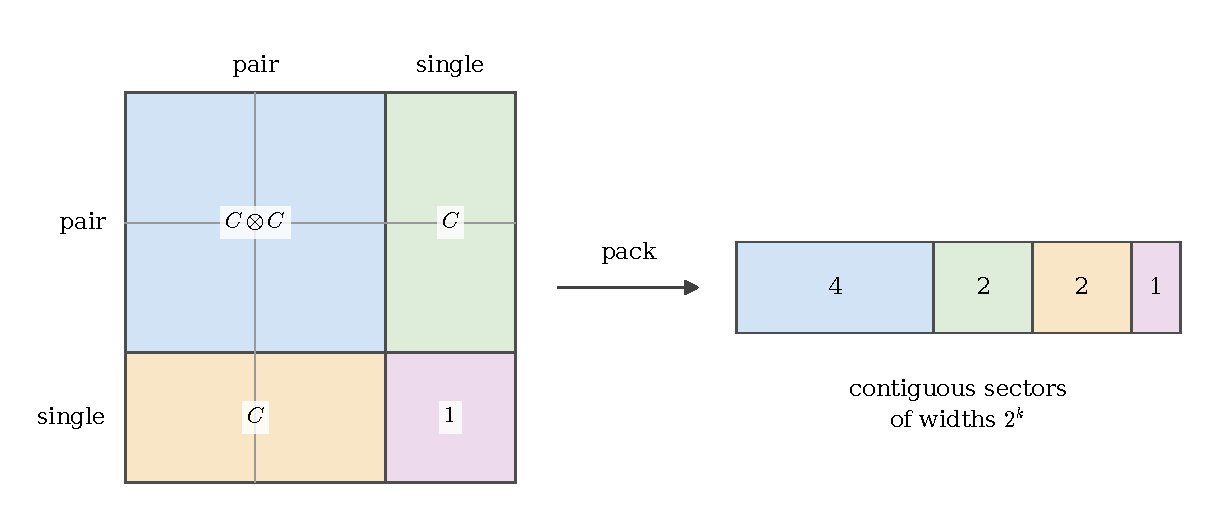
\includegraphics[width=.92\linewidth]{figures/sectors.pdf}
\caption{Two axes, each partitioned into a pair and a singleton. A simultaneous pair layer becomes four independent tensor-power calls. The original pair coordinates can be nonconsecutive; the local tables and~\eqref{eq:sector-updates} perform the reordering in linear time.}
\label{fig:sectors}
\end{figure}

\subsection{The synchronized transform}

\begin{samepage}
\begin{proposition}\label{prop:tensor-fourier}
Let $\ell\ge1$ and $r_1,\ldots,r_\ell\ge2$ be integers, and suppose
the required specified roots are given. Put $R=\prod_jr_j$ and
$r_{\max}=\max_jr_j$. The map $\bigotimes_jF_{r_j}$ is computable in
\begin{equation}\label{eq:tensor-fourier}
 O\!\left(R(\ell+1)^\theta(1+\log r_{\max})^4\right)
   +\poly(\ell,r_{\max},\log(R+2))
\end{equation}
operations, including compilation, scalar preparation, and array work. The polynomial and the implicit constant are absolute.
\end{proposition}
\end{samepage}
\begin{proof}
Use Proposition~\ref{loc:compiler} on every axis. Its words can be refined and padded to a common sequence of $O((1+\log r_{\max})^4)$ slot types: a monomial slot or a slot of disjoint copies of $C$ and singleton identities. Padding a pair slot means using only singleton blocks on that axis.

At each slot take the tensor product across axes. These slots multiply to the desired tensor transform because
\begin{equation}\label{eq:tensor-multiply}
 (\bigotimes_j A_j)(\bigotimes_j B_j)=\bigotimes_j(A_jB_j).
\end{equation}
In particular, a local word's correctness on arbitrary inputs suffices. Another axis may change coordinates during intermediate slots; one does not require it to preserve the local word's borrowed coordinates throughout that word.

Tensor monomials cost $O(R)$ by the prefix traversal. A tensor pair slot decomposes into the sectors of Lemma~\ref{lem:sector-address}. Its width-$2^k$ sector carries precisely $C^{\otimes k}$. Theorem~\ref{net:tensor-bound} bounds its cost, including invocation and movement, by $O(2^k(k+1)^\theta)$. As $k\le\ell$ and the sector widths sum to $R$, their total cost is $O(R(\ell+1)^\theta)$. Packing, unpacking, and discovering even the width-one sectors cost another $O(R)$. This proves the first term of~\eqref{eq:tensor-fourier}.

The local compilers use polynomial work in their widths. Suffix products, local block tables, and the other integer preparation use polynomial work in $\ell,r_{\max},\log(R+2)$. All running scalar products have been charged in the traversal, so the polynomial term describes local preparation only.
\end{proof}

\section{Working lengths and the transform at every length}
\label{sec:all-lengths}

To apply the synchronized transform at a requested length $n$, we first
choose a working length $L$ with $2n\le L<4n$. The lower bound permits
the chirp convolution below, while the upper bound keeps its array size
linear in $n$. We also need small coprime factors: their widths must be
polynomial in $\log n$ so that local compilation has only polylogarithmic
cost. A product of initial odd primes supplies these axes, and one
power of two fills the remaining gap to $2n$.

\subsection{Enough small, pairwise coprime factors}

Let $r_1<r_2<\cdots$ be the odd primes and let $R_\ell=\prod_{j=1}^{\ell}r_j$, with $R_0=1$. The modest estimate below suffices; no prime number theorem is used.

\begin{lemma}\label{lem:prime-lengths}
One has $r_j=O((j+1)^2)$ and
\[
 \log R_\ell=\Theta(\ell\log(\ell+2)).
\]
For the largest $\ell$ with $R_\ell\le2n$, as $n\to\infty$,
\begin{equation}\label{eq:axis-count}
 \ell=\Theta\!\left(\frac{\log n}{\log\log n}\right),
 \qquad \log\ell=\Theta(\log\log n).
\end{equation}
The primes and this value of $\ell$ can be found with a number of
operations polynomial in $\log(n+2)$, using $O(\log(n+2))$-bit integers.
\end{lemma}
\begin{proof}
Writing $\pi(t)$ for the number of primes at most $t$, for integer $u\ge1$ we have
\begin{equation}\label{eq:binomial-primes}
 \frac{4^u}{2u+1}\le\binom{2u}{u}\le(2u)^{\pi(2u)}.
\end{equation}
The first inequality follows because the central binomial coefficient is largest. In the factorial formula, the exponent of a prime $p$ in $\binom{2u}{u}$ is
\[
 \sum_{a\ge1}\bigl(\lfloor2u/p^a\rfloor-2\lfloor u/p^a\rfloor\bigr)
 \le\lfloor\log_p(2u)\rfloor.
\]
Its prime-power contribution is therefore at most $2u$, proving the second inequality. Taking $u=(j+1)^2$ shows that $\pi(2u)>j+1$ for all sufficiently large $j$, so the $j$th odd prime is $O((j+1)^2)$.

The upper bound on $\log R_\ell$ now follows by summation. For the lower bound, $r_j\ge j+2$, so $R_\ell\ge(\ell+2)!/2$. For instance, the last half of these factors alone give a constant times $\ell\log\ell$ in the logarithm. Maximality says
\[
 R_\ell\le2n<R_\ell r_{\ell+1}.
\]
The extra logarithm is $O(\log(\ell+2))$, giving $\log n=\Theta(\ell\log\ell)$ and hence~\eqref{eq:axis-count}.

Primes up to the first unused prime are bounded by a fixed polynomial in $\ell+1=O(\log(n+2))$. Testing potential divisors of each candidate is already polynomial work in $\log(n+2)$. Maintain the product and stop at the first exceeding $2n$; the product at stopping is at most $2n$ times a polynomial in $\log(n+2)$. All these integers have $O(\log(n+2))$ bits.
\end{proof}

Choose this $\ell$, and let $e\ge0$ be the least integer for which
\begin{equation}\label{eq:working-length}
 L=R_\ell2^e\ge2n.
\end{equation}
Then
\begin{equation}\label{eq:working-bounds}
 2n\le L<4n,\qquad 2^e<2r_{\ell+1},\qquad
 e=O(\log(\ell+2)).
\end{equation}
Bounded lengths can be treated directly, so subsequent asymptotic estimates may assume $\ell\ge1$.

\subsection{CRT permutations and the working transform}

We use Good's coprime tensor factorization~\cite[Section~12]{good1958},
with its index permutations included in the cost.

For pairwise coprime factors $q$ of $L$, here the odd primes and the factor $2^e$ when nontrivial, choose $d_q$ with
\[
 (L/q)d_q\equiv1\pmod q,
 \qquad E_q=(L/q)d_q.
\]
The integers $E_q$ are orthogonal idempotents modulo $L$. The Chinese remainder indexing
\[
 (j_q)_q\longmapsto \sum_q E_qj_q\pmod L
\]
is a bijection, and for similarly indexed $k$,
\begin{equation}\label{eq:crt-fourier}
 \zeta_L^{jk}=\prod_q\zeta_q^{d_qj_qk_q}.
\end{equation}
Thus, after permutations of the input and output indices, $F_L$ is the tensor product of the $F_q$. The local output permutation multiplies a digit by the unit $d_q$ modulo $q$.

These permutations take $O(L)$ array operations. Prepare the local tables $E_qa\bmod L$ and $d_qa\bmod q$, then enumerate digit tuples with an accumulated sum and mixed-radix address. The prefix bound~\eqref{eq:prefix-nodes} applies; no division by every factor is performed separately for each array entry. Computing the inverses $d_q$ and local tables is polynomial in the logarithm of $n$.

Apply Proposition~\ref{prop:tensor-fourier} on the odd-prime axes, with each digit of the power-of-two axis fixed in turn. Then apply the usual radix-two FFT on the fibers of that remaining axis. The former costs
\[
 O\!\left(L(\ell+1)^\theta(1+\log(\ell+2))^4\right)
   +\poly(\log(n+2)),
\]
because $r_\ell=O((\ell+1)^2)$; the latter costs $O(L(1+e))$. Local tables are shared among the fibers. The standard binary recursion uses $O(q\log(q+1))$ operations at length $q=2^e$, with $O(q)$ twiddle preparation and ordinary linear-time stage indexing. Here $q$ is only polynomial in $\ell+1$.

Consequently both $F_L$ and its inverse have total cost
\begin{equation}\label{eq:working-transform}
 O\!\left(L\bigl[(\ell+1)^\theta(1+\log(\ell+2))^4+1+e\bigr]\right)
   +\poly(\log(n+2))+O(1).
\end{equation}
For the inverse, the geometric root sum gives $F_L^2=LJ$, where $J$ negates indices modulo $L$. Thus $F_L^{-1}=L^{-1}JF_L$, with only linear additional work. The absolute term includes the fixed network construction.

\subsection{Chirp convolution and preparation}

The reduction is Bluestein's chirp convolution~\cite{bluestein}, in the
weighted-convolution form of~\cite[Section~II]{rabinerSchaferRader1969}.
We charge preparation of the fixed convolution operand explicitly.

Put $\eta=\zeta_{2n}$. For $0\le j,k<n$,
\begin{equation}\label{eq:chirp}
 \zeta_n^{jk}=\eta^{k^2}\eta^{-(k-j)^2}\eta^{j^2}.
\end{equation}
Prepare two length-$L$ vectors. The input-dependent vector has value $\eta^{j^2}x_j$ at $0\le j<n$ and zero elsewhere. The fixed vector has value $\eta^{-u^2}$ at the residues represented by $-(n-1)\le u\le n-1$, and zero elsewhere. These residues are distinct by $L\ge2n$. Cyclic convolution of the vectors therefore gives, at each $0\le k<n$, the sum in~\eqref{eq:chirp} before multiplication by $\eta^{k^2}$.

The convolution is obtained by applying $F_L$ to both vectors, multiplying pointwise, and applying $F_L^{-1}$. The transform of the fixed vector is part of scalar preparation and is explicitly charged as one full transform. Its pointwise use multiplies the variable data only by prepared scalars. Chirp tables and the zero-padded vectors take $O(L)=O(n)$ work: successive ratios of the chirps form a geometric progression, so no separate long exponentiation is needed at every entry. There are only three full transforms.

We now specify the single root promised in Theorem~\ref{thm:main}. With $L$ as in~\eqref{eq:working-length}, set
\begin{equation}\label{eq:master-root}
 D_*=(2n)L\,2^{\lceil\log_2(16L)\rceil}.
\end{equation}
The chirp root has order $2n$, and the working factor roots have orders dividing $L$. Proposition~\ref{loc:compiler} needs power-of-two roots of orders at most $8r$ for a local width $r\le L$; each such order divides the last factor in~\eqref{eq:master-root}. The fixed kernel uses only $i$ and rational constants. Thus every required initial root is an integer power of the supplied, specified $\zeta_{D_*}$. Moreover,
\begin{equation}\label{eq:root-size}
 D_*<64nL^2<1024n^3.
\end{equation}
Binary powering extracts each local initial root in $O(\log(n+2))$ field operations. There are polynomially many local constants and instructions in $\log(n+2)$, so all local extraction and compilation remain polynomial in that logarithm.

The local scalar programs are arithmetic DAGs with shared subexpressions.
As in Proposition~\ref{loc:compiler}, a coefficient's conjugate is prepared
by evaluating the same DAG with unchanged rational literals and inverse
Fourier roots, including $i^{-1}=-i$. Thus no conjugation of variable
input data or zero decision about complex coefficients is required.
Full-array scalar products and the transformed convolution kernel have
already been charged in~\eqref{eq:working-transform}; only the
\emph{local} preparation is polynomial in $\log(n+2)$.

\subsection{The final estimates}

\begin{proof}[Proof of Theorem~\ref{thm:main} and Corollary~\ref{cor:decimal}]
All maps in the construction are exact and deterministic. The local word compiler and the fixed finite network have specified finite construction procedures. On the input data the algorithm is linear, including the chirp reduction, since the second convolution operand is fixed.

By~\eqref{eq:working-bounds}, $e=O(\log(\ell+2))$ and $L=\Theta(n)$. Because $\theta>0$, equation~\eqref{eq:working-transform} and the constant number of transforms give
\[
 T(n)=O(n\ell^\theta(\log\ell)^4)
       +\poly(\log(n+2))+O(1).
\]
Every fixed power of $\log(n+2)$ is eventually negligible compared with $n\ell^\theta$. Substituting~\eqref{eq:axis-count} proves~\eqref{eq:main-bound}.

For an exact bound on the exponent, direct integer arithmetic in~\eqref{eq:main-constants} gives
\[
 \varepsilon:=\frac{\Delta}{mW_*}
   =\frac{1717850673}{590295810358705651712}
   >\frac{28}{10^{13}}.
\]
Since $\log m<14$, for $\eta_0=2/10^{13}$ one has $\eta_0\log m<\varepsilon$. Using $\exp(-t)\ge1-t$,
\[
 \lambda=m(1-\varepsilon)<m\exp(-\eta_0\log m)
       =m^{1-2\cdot10^{-13}}.
\]
Hence $\theta<1-2\cdot10^{-13}$. The fixed power of $\log\log n$ in~\eqref{eq:main-bound} is smaller than $(\log n)^{10^{-13}}$ for all sufficiently large $n$. This proves Corollary~\ref{cor:decimal}.

Finally, all lengths, root orders, products of indices, and addresses are polynomially bounded in $n$ with absolute constants;~\eqref{eq:root-size} treats the largest root order explicitly. Fixed network tables contribute absolute constants, and local tables have size polynomial in $\log(n+2)$. Array movement and traversal were counted in Theorem~\ref{net:tensor-bound} and Lemma~\ref{lem:sector-address}. Therefore a fixed number of $O(\log(n+2))$-bit words per integer suffices throughout, as required by the model.
\end{proof}

\subsection{Two-input convolution and polynomial multiplication}
\label{sec:convolution-consequence}

The chirp reduction above convolves input data with a fixed vector and
therefore remains linear. For two variable operands, the same Fourier
identity gives Corollary~\ref{cor:polynomial-multiplication}, with one
product of two input-dependent values at each transform coordinate.

\begin{proof}[Proof of Corollary~\ref{cor:polynomial-multiplication}]
Set $M=2n-1$ and zero-pad $a$ and $b$ to vectors $\widetilde a,\widetilde b$
of length $M$. Every sum of two indices in their supports lies between zero
and $2n-2=M-1$, so the length-$M$ cyclic convolution has no wraparound and
is exactly $(c_0,\ldots,c_{M-1})$. With the positive-exponent convention
for $F_M$, its convolution identity is
\[
 (F_Mc)_j
 =\sum_{r,s=0}^{n-1}a_rb_s\zeta_M^{j(r+s)}
 =(F_M\widetilde a)_j(F_M\widetilde b)_j
 \qquad(0\le j<M).
\]
Compute the two forward transforms and their $M$ pointwise products, obtaining
a vector $p=F_Mc$. If $J$ negates indices modulo $M$, the geometric root sum
gives $F_M^2=MJ$ and therefore
\[
 c=F_M^{-1}p=M^{-1}JF_Mp.
\]
Thus one more forward transform, index reversal, and scaling give the answer.

Apply Theorem~\ref{thm:main} at length $M$ for each of the three transforms,
charging its scalar preparation, schedule construction, and index work each
time. The single specified root supplied for that length can be reused in
all three calls. Its explicitly computable order satisfies
$D_*<1024M^3<8192n^3$; equivalently, the model's root-of-unity operation
returns this one root. Padding, pointwise products, reversal, and output
scaling take $O(M)$ field and address operations. To prepare $M^{-1}$,
form the complex integer $M$ from $1$ by binary doubling and addition in
$O(\log(M+2))$ field operations, then divide $1$ by it; the denominator is
nonzero because $M\ge1$. All added indices and addresses fit a fixed number
of $O(\log(n+2))$-bit words.

If $T(M)$ denotes the charged running time in Theorem~\ref{thm:main}, the
total is $3T(M)+O(M+\log(M+2))$. Since $M=\Theta(n)$, this gives the first
bound, and Corollary~\ref{cor:decimal} gives the eventual decimal power bound.
The same formulas apply when $n=1$; a finite initial range may also be handled
directly.
\end{proof}

\appendix
\section{Effective synthesis and uniform compilation}
\label{syn:section}
\label{sec:synthesis}

This appendix gives a general route from a finite tensor saving to a
uniform Fourier algorithm.  Its purpose is to separate two questions:
how to obtain usable coefficients from an existence theorem over $\C$,
and how to use effective small circuits when their compilation time has
no useful bound.  The explicit network in the main argument gives the
stronger quantitative conclusion without this search.
We first replace a complex certificate by identities in a fixed
finite-dimensional rational algebra.  Matrix representations of that
algebra then give ordinary scalar circuits without choosing a complex
embedding.  We print those circuits together with their scalar
preparation programs, and finally limit the printer's running time to
select a sufficiently small compiled radix for each input length.

The certificate used below consists of two finite words for the same
invertible nonmonomial matrix $A\in\GL_q(\C)$, with integers
$q,b\ge2$. The first word acts on exactly
$q^b$ coordinates as $A^{\otimes b}$ and uses
\begin{equation}\label{syn:win}
 g<bq^{b-1}
\end{equation}
forward calls to $A$, interspersed with invertible monomials. A call
acts on an ordered $q$-tuple and fixes every other coordinate. The
second word acts on $q$ coordinates as $U=I_q+E_{12}$, where $E_{12}$
is a matrix unit, using a positive number of forward calls to that same
$A$ and invertible monomials.

The companion paper~\cite[Theorem~8.3 and Lemma~2.2]{exactfourier}
obtains such a pair from a general finite-win theorem and positive
generation by an invertible nonmonomial matrix. The following lemma
supplies the particular certificate needed here directly from our
network. Thus the search-termination proof is also available locally.
The extraction and printer constructions that follow use only the two
word identities, so they retain their general certificate interface.

\begin{lemma}[A local certificate for the symbolic search]
\label{syn:local-certificate}
For the invertible nonmonomial matrix $C$ in \eqref{net:C}, there are
integers $b\ge2$ and $g\ge0$ and a word on exactly $2^b$ coordinates
which implements $C^{\otimes b}$ using $g<b2^{b-1}$ forward calls to
$C$ and invertible monomials. On two coordinates, $I_2+E_{12}$ has a
word with exactly three forward calls to the same $C$ and invertible
diagonal factors.
\end{lemma}

\begin{proof}
Use Proposition~\ref{net:finite-interface} and the padding
\eqref{net:padding} on $W_*=2^{71}$ arrays of length $2^{mf}$.
The $S=W_*m-\Delta$ directional steps require exactly
$Sf2^{mf-1}$ forward $C$-calls when their tensor factors are
applied separately: one step has $2^{(m-1)f}$ fibers, each requiring
$f2^{f-1}$ calls. Inverse steps add only translations.
Each scalar row of \eqref{net:schedule} is a composition of elementary
shears between existing, distinct roles; its source coordinates are
unchanged within that row. The coefficients are nonzero rational
numbers. Equation~\eqref{loc:nonzero-shear} therefore bounds the
pointwise work by $H2^{mf}$ forward calls for a fixed integer $H$
independent of $f$. All remaining operations are invertible monomials.
Every role carries arbitrary data, so this word uses exactly
$W_*2^{mf}$ coordinates and acts as
$I_{W_*}\otimes C^{\otimes mf}$. Address permutations here are
monomial factors on these coordinates; no implementation buffer is
added to the word's width.

Identify the role index with 71 binary axes and apply $C$ along
each of them. This costs $71W_*2^{mf-1}$ calls and gives
$C^{\otimes b}$ with $b=mf+71$. Its actual number $g$ of forward calls
therefore satisfies
\[
 g\le (Sf+71W_*+2H)2^{mf-1}
   =b2^{b-1}-(\Delta f-2H)2^{mf-1}<b2^{b-1}
\]
for any integer $f>2H/\Delta$.
Finally, $\det C=i$ and both scalar coefficients in \eqref{net:C} are
nonzero, so $C$ is invertible and nonmonomial.
Equation~\eqref{loc:nonzero-shear} with $t=1$ supplies the claimed
three-call word for $I_2+E_{12}$. Any embedded call on an ordered pair
is a permutation conjugate of $C\oplus I_{2^b-2}$; the permutations
can be absorbed into adjacent monomial factors.
\end{proof}

\subsection{Obtaining finite rational algebra data}

The extraction uses the triangular monic substitution from the standard
proof of Noether normalization~\cite[Tags 051M, 051N, and 00OX]{stacksNormalization}
and the determinant form of Nakayama's lemma~\cite{stacksNakayama}.
We give the rational algorithm and its termination proof in full.

\begin{lemma}[Effective finite algebra extraction]\label{syn:extraction}
Given finitely many polynomials $f_i$ in $a$ variables over $\Q$, a
deterministic rational algorithm either certifies that $(f_i)$ is the
unit ideal or produces a nonzero finite-dimensional commutative unital
$\Q$-algebra $E$, with a rational multiplication table, and elements
$\xi_1,\ldots,\xi_a\in E$ satisfying every $f_i(\xi)=0$.
In particular, a complex solution guarantees the second outcome.
Required units can be imposed by adding inverse-witness equations.
\end{lemma}

\begin{proof}
Keep a finite generating list for the ideal $I=(f_i)$ and an integer $m$,
initially $m=a$.  Retain polynomial-combination witnesses for derived
members of $I$; rational elimination and the monic reductions below
can track these witnesses.
After invertible polynomial changes of coordinates, maintain, for
each $j>m$, a known member of $I$ of the form
\[
 x_j^{d_j}+\sum_{e<d_j}c_{je}(x_1,\ldots,x_{j-1})x_j^e,
 \qquad d_j\ge1.
\]
Thus $S=\Q[x_1,\ldots,x_a]/I$ is finite as a module over
$R=\Q[x_1,\ldots,x_m]$.

First compute the fiber $S/(x_1,\ldots,x_m)S$.  This is effective:
set $x_1=\cdots=x_m=0$ and let $B$ be the quotient by only the
displayed monic relations.  As a tower of monic extensions, $B$ has
a rational basis consisting of the monomials whose $x_j$-exponents
are less than $d_j$ for $j>m$.  Successive monic reduction gives its
multiplication table.  If $\bar f_i$ are the images in $B$ of the
generators of $I$, form the rational span of all $b\bar f_i$ with
$b$ in this basis.  Since the basis spans $B$, this is exactly the
ideal $\sum_i B\bar f_i$.  Its quotient is the required fiber, so
rational linear algebra computes the fiber and its table.  A nonzero
fiber is the requested answer, after undoing the coordinate changes.
If $m=0$ and the fiber is zero, then $S=0$, so $I$ is the unit ideal.

Suppose the fiber is zero and $m>0$.  We claim $I\cap R\ne0$.
Otherwise $R\hookrightarrow S$.  Localize at
$\mathfrak m=(x_1,\ldots,x_m)$ in $R$.  The resulting finite
$R_{\mathfrak m}$-module $S_{\mathfrak m}$ is nonzero, since it still
contains $R_{\mathfrak m}$.  The zero fiber would give
$S_{\mathfrak m}=\mathfrak mS_{\mathfrak m}$.  For a finite generating
column $v$ this means $v=Mv$ with all entries of $M$ in the maximal
ideal.  Multiplication by the adjugate of $I-M$ gives
$\det(I-M)v=0$; its determinant is a unit, a contradiction.

Find a nonzero member $h\in I\cap R$ by enumerating increasing degree
cutoffs for monomial multiples of the generators of $I$.  At each
cutoff, rational linear algebra tests whether their span has a
nonzero element involving only the first $m$ variables.  This search
terminates by the claim and the definition of an ideal.  A nonzero
constant certifies $I=(1)$.  Otherwise let $d=\deg h\ge1$ and substitute
\[
 x_i=y_i+y_m^{(d+1)^i}\quad(1\le i<m),\qquad x_m=y_m,
\]
leaving later variables unchanged.  This change is invertible.
The weights $1,(d+1),\ldots,(d+1)^{m-1}$ distinguish all monomials of
total degree at most $d$ by base-$(d+1)$ expansion.  Consequently the
highest power of $y_m$ in the transformed $h$ has a nonzero rational
leading coefficient: it comes from a unique monomial, taking the
pure-power term in every substituted factor.  Divide by that
coefficient to obtain a monic relation in $y_m$.  Earlier triangular
relations remain monic in their respective later variables.  Rename
the variables and decrease $m$ by one.  At most $a$ such decreases
occur, proving termination.  Every step uses finite rational
arithmetic.  Finally, the equation $uv=1$ forces $u$ to be a unit in
every output algebra, including one with zero divisors.
\end{proof}

Enumerate integer tuples $(q,b,g,h)$ with $q,b\ge2$, $g\ge0$, $h\ge1$ and
\eqref{syn:win}.  For each tuple form polynomial equations for
\begin{equation}\label{syn:certificate}
 A^{\otimes b}=M_0YM_1Y\cdots YM_g,
 \qquad U=N_0AN_1A\cdots AN_h,
 \qquad Y=A\oplus I_{q^b-q}.
\end{equation}
All embedded placements are absorbed into adjacent monomials.
Include a matrix inverse witness for $A$.  In a monomial slot write
a variable permutation factor $P$ and a variable diagonal factor;
impose $p_{ij}^2=p_{ij}$ and row and column sums equal to $1$ on $P$,
and give every diagonal entry an inverse witness.  These are finite
polynomial systems over $\Q$.  Apply Lemma~\ref{syn:extraction} in a
fixed enumeration order until one succeeds.  Lemma~\ref{syn:local-certificate} gives a complex solution for a tuple
with $q=2$ and $h=3$, so success is guaranteed.

The entries $p_{ij}$ in the resulting $E$ may be nonscalar idempotents.
Resolve them one at a time.  For a current idempotent $p\ne0$, replace
$E$ by the nonzero algebra $pE$ with unit $p$ and project every stored
element by $z\mapsto pz$; if $p=0$, do nothing.  This is a unital
homomorphism onto the new algebra and makes the current idempotent
equal to its unit.  Previously resolved values remain $0$ or $1$.
After finitely many rational table operations all permutation entries
are $0$ or $1$, and their row and column sums give actual permutations.
All identities, inverse witnesses, and diagonal units survive.
Choose a rational basis of the final nonzero algebra beginning with
$1_E$.  We have thus computed fixed, fully specified data
\eqref{syn:certificate} over $E$.

\begin{remark}[Faithful scalar simulation]\label{syn:simulation}
If $d=\dim_{\Q}E$, then $E\otimes_{\Q}\C$ is the vector space $\C^d$
with the computed multiplication table.  The embedding
$z\mapsto z1_E$ is injective.  Addition is coordinatewise and
multiplication by any prepared algebra element is a $d\times d$
complex matrix, so each linear algebra operation costs $O(d^2)$
ordinary scalar operations.  When a circuit acts as $F_r$ times the
algebra identity, embed its inputs as multiples of $1_E$ and read the
first coordinate of each output.  This is a faithful, constant-factor
simulation; choosing a complex embedding or extracting algebraic
roots is unnecessary.  Here $d$ is fixed before the input length is
known.
\end{remark}

\subsection{A printer for increasingly efficient radices}

We record why the fixed identities suffice for an effective circuit
printer.  The tensor amplification of \cite[Lemma~2.3]{exactfourier}
also works over $E$: its proof uses only the identities and linear
operations.  Explicitly, put $Q=q^b$, $j=\lfloor k/b\rfloor$ and
tensor the first word in \eqref{syn:certificate} across $j$ groups.
Every call slot decomposes, after reindexing, as
\[
 (A\oplus I_{Q-q})^{\otimes j}
 \cong\bigoplus_{r=0}^j
 (A^{\otimes r})^{\oplus\binom jr(Q-q)^{j-r}}.
\]
Recurse on these smaller tensor orders and use direct calls on the
fewer than $b$ remaining axes.  Monomial scalings and copies cost
linear size at each level.  Let $f(k)$ be the size of this recursive
construction divided by $q^k$.  The total width of the sectors with
$r$ active factors, divided by $Q^j$, is
\[
 \frac{\binom jr(Q-q)^{j-r}q^r}{Q^j}
 =\binom jr(q/Q)^r(1-q/Q)^{j-r}.
\]
Thus the normalized cost satisfies
\[
 f(k)\le C_0+g\,\mathbb E f(K),\qquad
 K\sim\operatorname{Bin}(\lfloor k/b\rfloor,q/Q).
\]
The distribution weights sectors by their dimensions.  Since
$gq/(bQ)<1$, choose $0<\alpha<1$ with
$g(q/(bQ))^\alpha<1$.  Concavity and induction, using
$\mathbb E(K+1)^\alpha\le(1+kq/(bQ))^\alpha$, give
\begin{equation}\label{syn:amplification}
 f(k)=O((k+1)^\alpha).
\end{equation}
The strict inequality absorbs $C_0$ for large $k$; enlarge the
inductive constant for the finite initial range.  Neither $\alpha$
nor that constant is needed by the printer.

For successive $t\ge1$, let $r_1<\cdots<r_t$ be the first $t$ primes
greater than $2q$, and put
\[
 m_t=\prod_{i=1}^t r_i,\qquad
 \ell_t=m_t\,2^{\lceil\log_2(16r_t)\rceil},\qquad
 R_t=\Q[z]/(\Phi_{\ell_t}(z)).
\]
Cyclotomic polynomials and arithmetic in this finite algebra are
effective: compute $\Phi_s$ recursively from
$z^s-1=\prod_{d\mid s}\Phi_d(z)$, and use polynomial division and
the Euclidean algorithm.  A polynomial is a unit modulo $\Phi_s$
exactly when their gcd is $1$.  The distinct roots of $\Phi_s$ are
the primitive $s$th roots, so identities in $R_t$ can be checked at
all primitive specializations.  Roots of orders dividing $\ell_t$
are compatible powers of $z$.
Carry out the next constructions over $E\otimes_{\Q}R_t$, with the
Fourier coefficients in the central factor $R_t$.  The two certificate
identities and their inverse witnesses persist under extension of
scalars; in particular, every certified unit remains a unit.

Use the exact-width Fourier layer construction of Lemma~\ref{loc:fourier}
on each width $r_i$.  It gives $O(1+\log^4 r_t)$ monomial or disjoint
shear layers.  Its rational formulas hold in $R_t$: all denominators
are nonzero at every primitive specialization, and the convolution
root orders divide the indicated power of two.  In particular the
Newton denominators $\prod_{a=1}^j(1-u^a)$ have $j<r_i$ for a
primitive $r_i$th root $u$.  The measured workspace test is a test on
the integer circuit description and is unchanged by this scalar
extension.

To substitute the second word of \eqref{syn:certificate}, split any
shear coefficient $c\in R_t$ into two units $d+(c-d)$, where $d$ is
a positive integer chosen by testing $d=1,2,\ldots$ until $c-d$ is a
unit.  This terminates: only finitely many complex values of $c$ at
the primitive roots can be positive integers.  A shear with a unit
coefficient $v$ is obtained by conjugating $U$ by
$\diag(v,1,\ldots,1)$, so it has the fixed word pattern from
\eqref{syn:certificate}.  The resulting word restores the arbitrary values of
its $q-2$ spectator coordinates.  Partition the disjoint pairs of an
axis into at most $q$ batches of at most $\lfloor r_i/q\rfloor$ pairs;
this is possible because $r_i>2q$ gives
$q\lfloor r_i/q\rfloor\ge\lfloor r_i/2\rfloor$.
Each batch fits disjoint $q$-tuples inside the same $r_i$ coordinates.
Its spectators may belong to other pairs, since they are restored
before the next batch.

Synchronize these fixed word patterns across axes, with identities
in idle positions.  Their product is the tensor of the local products
by the tensor multiplication identity.  Each monomial slot has linear
size.  Every other slot is a direct sum of $A^{\otimes k}$ with
$k\le t$ and total width $m_t$, so \eqref{syn:amplification} bounds
its size by $O(m_t(t+1)^\alpha)$.  Chinese remainder reindexing gives
$F_{m_t}$ from the tensor of the local Fourier transforms.
Now specialize $R_t$ by $z\mapsto\zeta_{\ell_t}$, obtaining a circuit
over $E\otimes_{\Q}\C$ whose output matrix is $F_{m_t}$ times the
algebra identity.  Expand only the fixed algebra $E$ by
Remark~\ref{syn:simulation}.  Its dimension contributes a constant
factor, whereas $R_t$ has supplied polynomial expressions for the
complex coefficients.  The resulting complex linear circuit has size
\begin{equation}\label{syn:radix-size}
 s_t=O\bigl(m_t(t+1)^\alpha(1+\log^4(t+2))\bigr)
     =o(m_t\log m_t).
\end{equation}
Here $r_t=O_q((t+1)^2)$, by the elementary prime estimate in
Lemma~\ref{lem:prime-lengths}, and $\log m_t\ge t\log2$.  The printer computes all
tensor coefficients and all wiring explicitly.  It may take any
finite amount of bit computation to do so.  Each coefficient is a
polynomial with rational coefficients evaluated at
$\zeta_{\ell_t}$; symbolic inverses have already been reduced in
$R_t$.  For each polynomial coefficient, print a finite Horner evaluation list,
with its rational literals written explicitly; sharing previously computed
values is optional.  Thus the printed record contains a complete circuit
and a fully expanded scalar preparation program, with no unspecified
complex constants or hidden loops.

\subsection{From a slow printer to a fast uniform algorithm}

\begin{theorem}[Bounded-printer uniformization]\label{syn:printer}
Suppose a fixed bit machine prints a sequence of complete records
$(m_t,C_t)$ with strictly increasing $m_t\to\infty$, where $C_t$
computes $F_{m_t}$ by $s_t=o(m_t\log m_t)$ scalar linear gates.
Each record must explicitly list the gates, output indices, and a
scalar preparation program with every instruction explicitly listed
and executed once in order.  Its instructions use rational literals, field
operations with valid nonzero divisors, and canonical Fourier roots
$\zeta_a=\exp(2\pi i/a)$ of positive integer orders
whose orders are written literally in binary.  Then there is one
deterministic algorithm computing every $F_n$ in $o(n\log n)$ time,
including preparation and indexing in the model of this paper.
A single specified root of order less than $8n^3$ suffices.
\end{theorem}

\begin{proof}
The printing budget will control both the circuit description and all
literal scalar data, without requiring a bound on when a record appears.
Normalize the printer to output at most one bit per machine step.
For $n\ge2$, run it from the beginning for
$B=\lfloor\log_2 n\rfloor$ bit steps.  Select the last completed
record with $2\le m_t\le\sqrt B$; if there is none, use the ordinary radix
$m=2$ circuit.  Every fixed record eventually finishes and satisfies
the width bound, so the selected stream index tends to infinity.
In particular $m\to\infty$ and $s/(m\log m)\to0$.

The total visible description has at most $B$ bits.  Decode the
selected explicit lists to addressable arrays and evaluate its
preparation program once.  Construct rational literals by their
binary expansions and perform each listed operation in the stated
arithmetic model.  This costs $B^{O(1)}$, including parsing and bit
simulation.  The gate list then executes on each new input in
$O(m+s)$ time, including entry and output copies.  There is no
expansion of a succinct circuit during its invocation.

Put $X=2n-1$, let $m^H$ be the largest power of $m$ not exceeding
$X$, and set
\[
 p=\lceil X/m^H\rceil,\qquad P=m^Hp.
\]
Then $1\le p\le m$, $X\le P<2X<4n$, and
$H\le\log(2n)/\log m$.  The mixed-radix Fourier recursion uses $H$
copies of radix $m$ and one radix $p$, the latter computed directly.
For clarity, at a split $ab$ use input index $bj_a+j_b$ and output
index $k_a+ak_b$.  The identity
\[
 (bj_a+j_b)(k_a+ak_b)
 \equiv bj_ak_a+aj_bk_b+j_bk_a\pmod {ab}
\]
gives the two smaller Fourier transforms and their intervening
twiddle.  At each level, copying subarrays into the required order,
tabulating or reading twiddles, and enumerating the two indices cost
linear work.  Reuse the decoded radix circuit each time.  Tabulate
powers of $\zeta_P$ in $O(P)$ operations; every recursive width
divides $P$.  Thus one transform, or its inverse by frequency
reversal and scaling, costs
\begin{equation}\label{syn:uniform-cost}
 O\bigl(P[1+p+H(1+s/m)]\bigr)+B^{O(1)}.
\end{equation}
All indices and products of indices have polynomial bounds in $n$,
so a constant number of $O(\log(n+2))$-bit words suffices per access.

Finally reduce $F_n$ to convolution of length $P$.  With
$\eta=\zeta_{2n}$, store $\eta^{j^2}x_j$ for $0\le j<n$ and pad
with zeros.  The fixed kernel stores $\eta^{-h^2}$ at the residues
of $-(n-1)\le h\le n-1$; these residues are distinct since
$P\ge2n-1$.  Multiply convolution output $k$ by $\eta^{k^2}$.
The identity $k^2+j^2-(k-j)^2=2kj$ gives exactly $F_nx$.
Computing the fixed kernel's transform, the variable transform and
the inverse uses only a constant number of transforms bounded by
\eqref{syn:uniform-cost}, plus linear preparation and scaling work.
The chirp scalars come from an $O(n)$-size table of powers of $\eta$,
indexed by the squared exponents modulo $2n$.

For the root accounting, let $R$ be the product of the root orders
listed in the selected preparation program, or $1$ if there are
none.  Their total binary length is at most $B$, whence
$R\le2^B\le n$.  The single root
$\zeta_D$, where $D=2nPR<8n^3$, supplies every listed root and the
two outer roots by integer powering.  There are at most $B$ such
requests, and powering and forming their exponents cost $B^{O(1)}$.
This includes obtaining the required powers of the supplied root in the
preparation bound.

Since $p=O(1+\sqrt{\log n})$, dividing the arithmetic term of
\eqref{syn:uniform-cost} by $n\log n$ gives
\[
 O\left(\frac{1+p}{\log n}
       +\frac1{\log m}+\frac{s}{m\log m}\right)=o(1).
\]
The polynomial logarithmic preparation term is also $o(n\log n)$.
Length $1$ is the identity.  This proves the claim, with all choices
independent of the input values.
\end{proof}

Applying Theorem~\ref{syn:printer} to the printer above yields a
uniform all-length $o(n\log n)$ algorithm directly from the finite
certificate interface.  The symbolic search, finite algebra, and stored
circuits are implementation devices; the only supplied complex
primitive is the explicitly specified Fourier root.  This conclusion
complements the explicit quantitative construction of the main text.

\clearpage
\begingroup
\raggedright
\bibliographystyle{plain}
\bibliography{references}
\endgroup
\end{document}
